\documentclass[usenatbib,a4paper,times,fleqn]{mnras}

\usepackage{aas_macros}
\usepackage{amsmath}
\usepackage{amssymb}
\usepackage{bm}
\usepackage{breakurl}
\usepackage{graphicx}
\usepackage{grffile}
\usepackage{natbib}
\usepackage{times}
\usepackage{textcomp}
\usepackage{url}

\newcommand{\todo}[1]{{\textcolor{red}{\bf[~TODO:\@ #1~]}}}
\newcommand{\newtext}[1]{{\textcolor{magenta}{#1}}}
\newcommand{\checkthis}[1]{{\textcolor{green}{#1}}}

\newcommand{\st}{\mathrm{St}}
\renewcommand{\sun}{\mathrm{M}_{\odot}}
\renewcommand{\earth}{\mathrm{M}_{\oplus}}
\newcommand{\mcfost}{\textsc{mcfost}}
\renewcommand{\phantom}{\textsc{phantom}}

\title[TW~Hya]{TW~Hya paper supplement}

\author[Mentiplay]{\parbox{\textwidth}{Daniel Mentiplay}}

\pagerange{\pageref{firstpage}--\pageref{lastpage}} \pubyear{2018}

\date{}


\begin{document}
\maketitle


\section*{Issues in \mcfost{} SPH interpolation (\texttt{2017-07-20})}

See Fig.~\ref{fig:voro-inner-region} for issues with Voronoi interpolation in
the inner disc where the particle density is low. See
Fig.~\ref{fig:dust-in-cell} for issues with the dust mass per grain size
interpolation in \mcfost{}.

\begin{figure}
   \begin{center}
      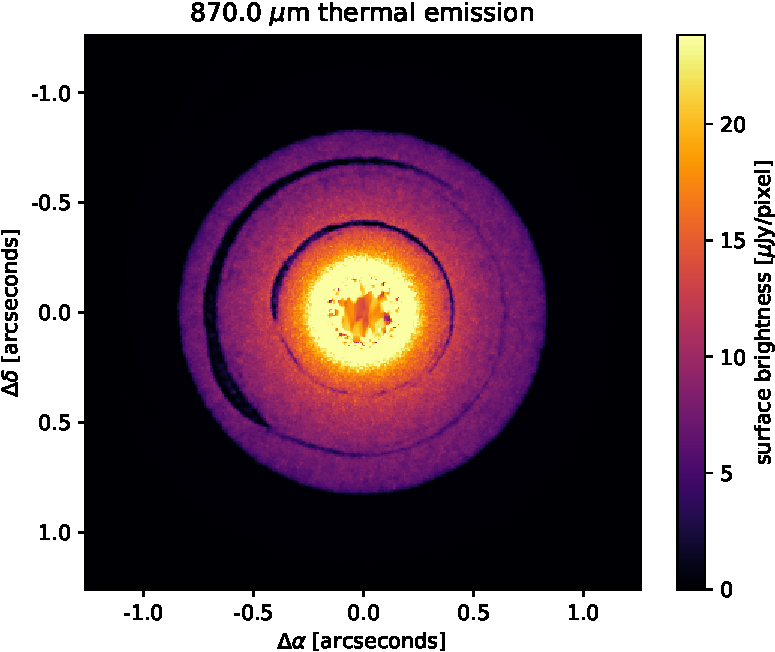
\includegraphics[width=0.48\columnwidth]{figs/dust-interpolation-inner-region-faceon.pdf}
      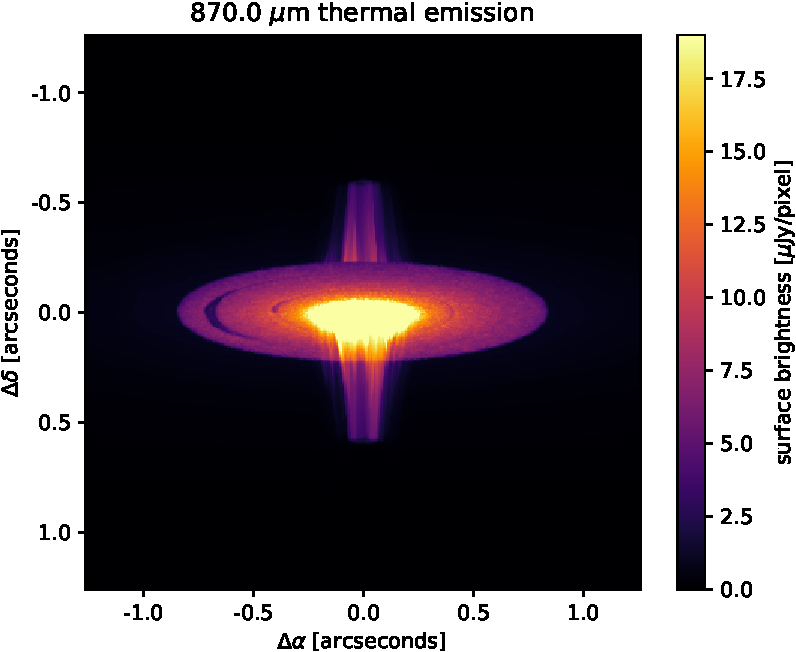
\includegraphics[width=0.48\columnwidth]{figs/dust-interpolation-inner-region-incl75.pdf}
      \caption{Dust interpolation in inner region: inner region is not well
      represented by Voronoi cells. Can see large vertical extent of cells in
      inclined image (\textit{right}). From \texttt{2017-05-30b/00090}. Note SPH
      dust mass is 5\% of total.}
      \label{fig:voro-inner-region}
   \end{center}
\end{figure}

\begin{figure}
   \begin{center}
      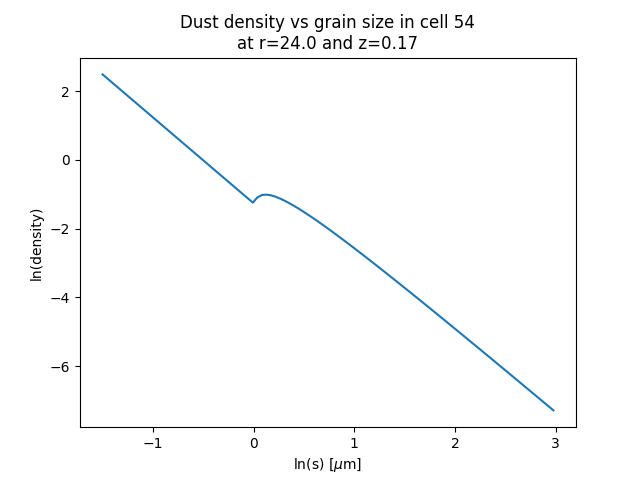
\includegraphics[width=0.32\columnwidth]{figs/dust-size-distribution-24.png}
      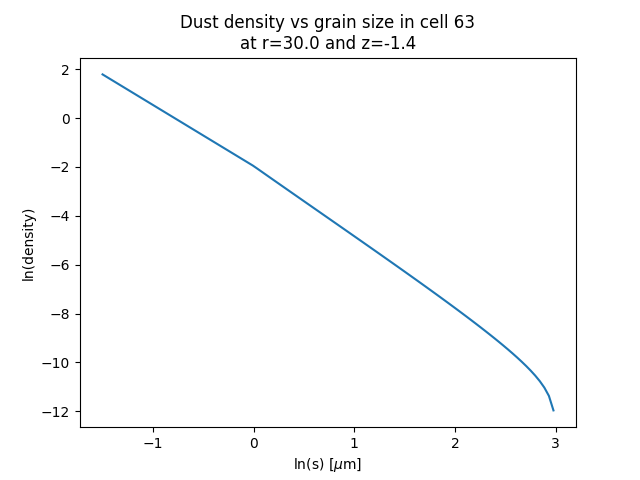
\includegraphics[width=0.32\columnwidth]{figs/dust-size-distribution-30.png}
      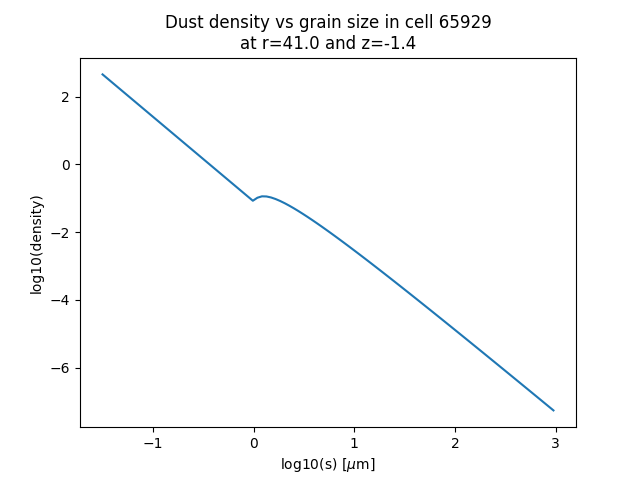
\includegraphics[width=0.32\columnwidth]{figs/dust-size-distribution-41.png}
      \caption{Dust vs size for a cell at 24~au (left), 30~au (center), and
         41~au (right). What are these weird bumps?}
      \label{fig:dust-in-cell}
   \end{center}
\end{figure}

\section*{Settling with 2-fluid dust (\texttt{2017-07-20})}

Dust seems to settle almost instantly with 2-fluid dust near $\st{}\sim 1$
(Fig.~\ref{fig:dust-settling}).

\begin{figure}
   \begin{center}
      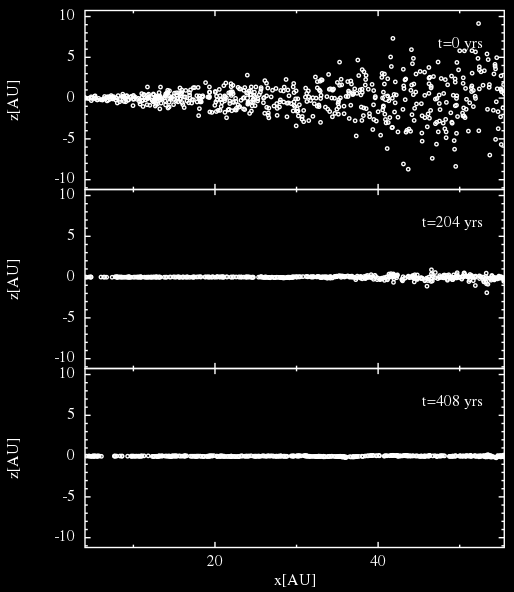
\includegraphics[width=0.95\columnwidth]{figs/settling-St-3e-1.png}
      \caption{Settling at $\st{} = 0.3$. Dust settles quickly. No need to
      pre-settle disc. However, this is $\st{}\sim 1$.}
      \label{fig:dust-settling}
   \end{center}
\end{figure}

\section*{Artificial viscosity and accretion in the inner disc
(\texttt{2017-07-20})}

Low resolution in the inner disc leads to high $\alpha$-viscosity and thus high
accretion. See Fig.~\ref{fig:artificial-viscosity}.

\begin{figure}
   \begin{center}
      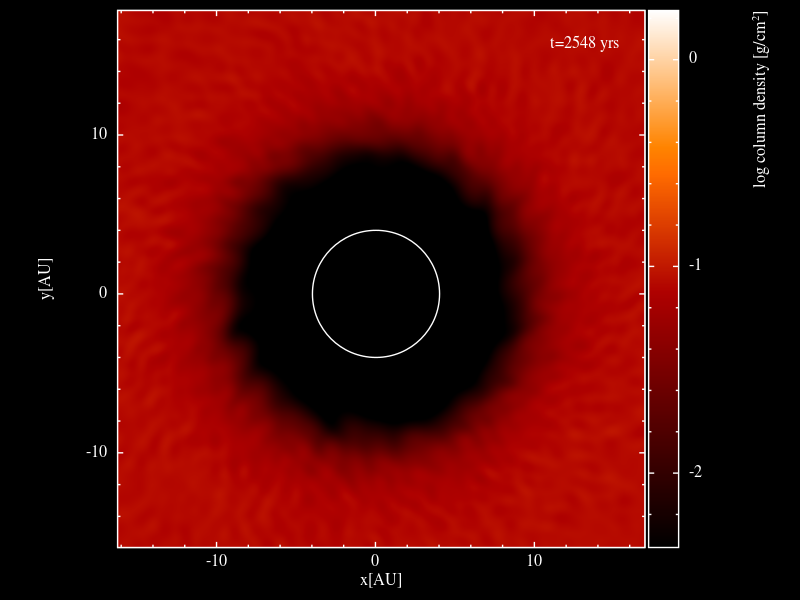
\includegraphics[width=0.48\columnwidth]{figs/artificial-viscosity-1e-1.png}
      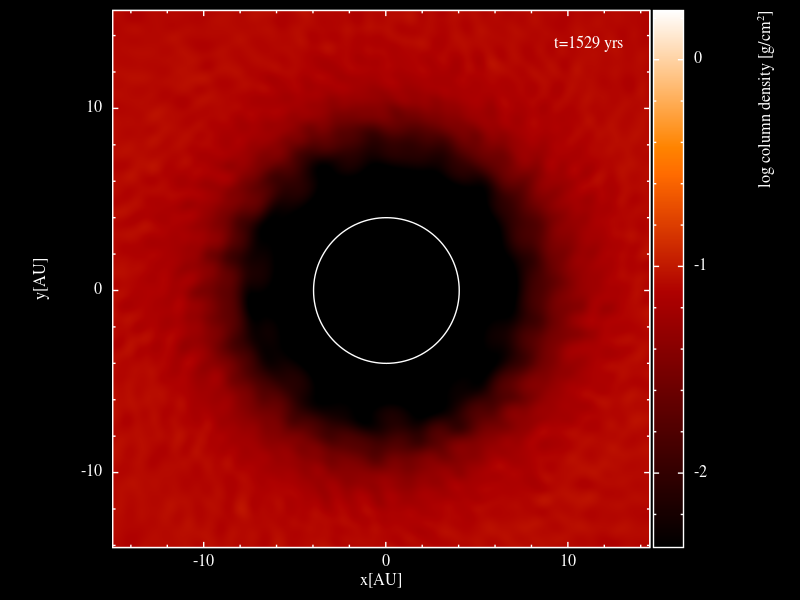
\includegraphics[width=0.48\columnwidth]{figs/artificial-viscosity-noDDISC_VISCOSITY.png}
      \caption{Artificial viscosity: changing this parameter has little effect
         on accretion onto the sink. \textit{Left}: $\alpha_{\mathrm{AV}}=0.1$;
         \textit{right}: no disc viscosity, i.e. without
         \texttt{DDISC\_VISCOSITY} flag. The point is that there doesn't seem to
         be much difference. Stick with $\alpha_{\mathrm{AV}}=0.1$ in the
      future.}
      \label{fig:artificial-viscosity}
   \end{center}
\end{figure}


\section*{Noise in simulated ALMA images in CASA (\texttt{2017-07-24})}

Noisier CASA images due to varying the precipitable water vapour
(Fig.~\ref{fig:pwv}), bin size of simulated grains, i.e. the ratio of simulated
dust mass to total dust mass (Fig.~\ref{fig:sph-dust-mass}), and beam size in
ALMA cycle (Fig.~\ref{fig:beam-size}).

\begin{figure}
   \begin{center}
      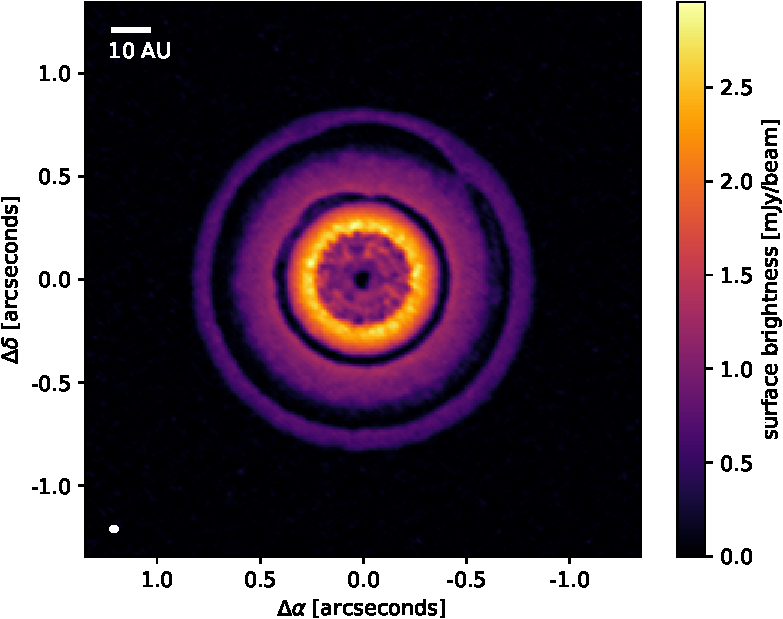
\includegraphics[width=0.48\columnwidth]{figs/pwv_1.0.pdf}
      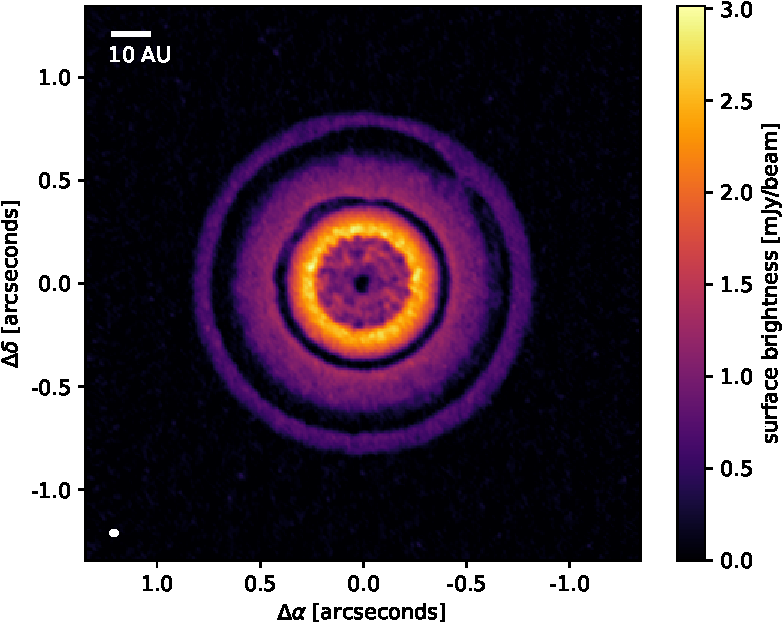
\includegraphics[width=0.48\columnwidth]{figs/pwv_2.0.pdf}\\
      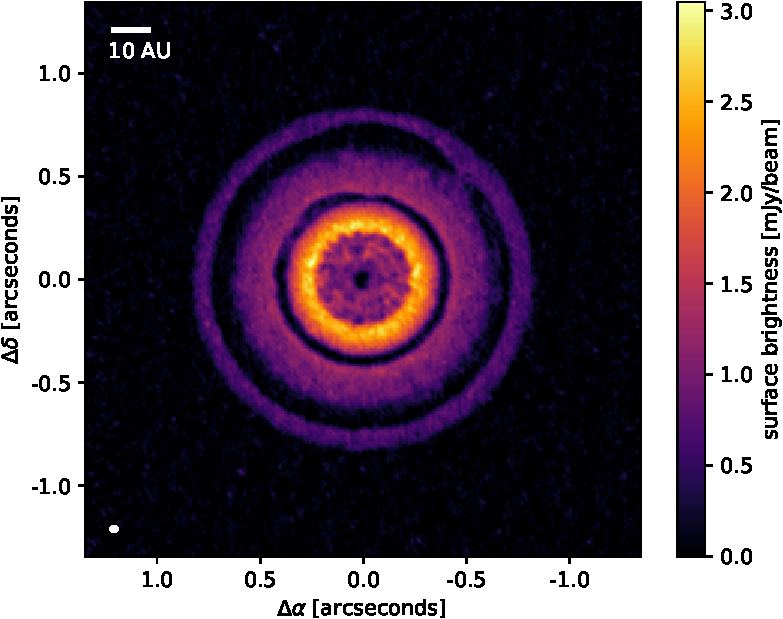
\includegraphics[width=0.48\columnwidth]{figs/pwv_3.0.pdf}
      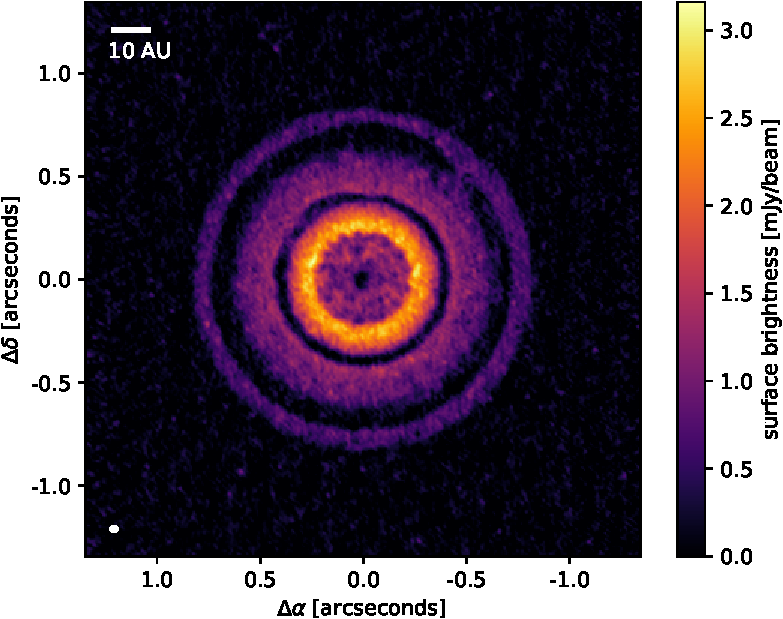
\includegraphics[width=0.48\columnwidth]{figs/pwv_5.0.pdf}
      \caption{Precipitable water vapour (PWV)\@: $1.0$, $2.0$, $3.0$, $5.0$
      from \texttt{2017-06-27a}, cycle 3.8, 45 minute observing time.}
      \label{fig:pwv}
   \end{center}
\end{figure}

\begin{figure}
   \begin{center}
      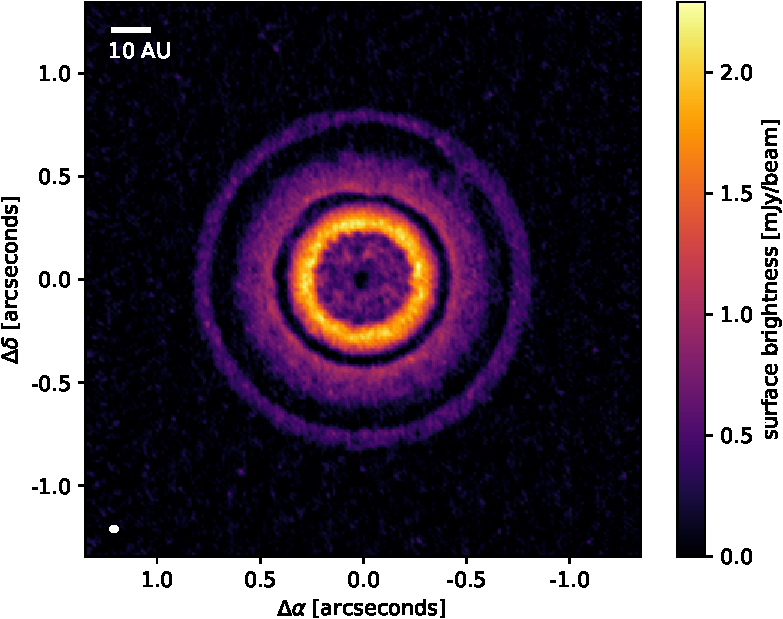
\includegraphics[width=0.32\columnwidth]{figs/total-to-SPH-dust_10.pdf}
      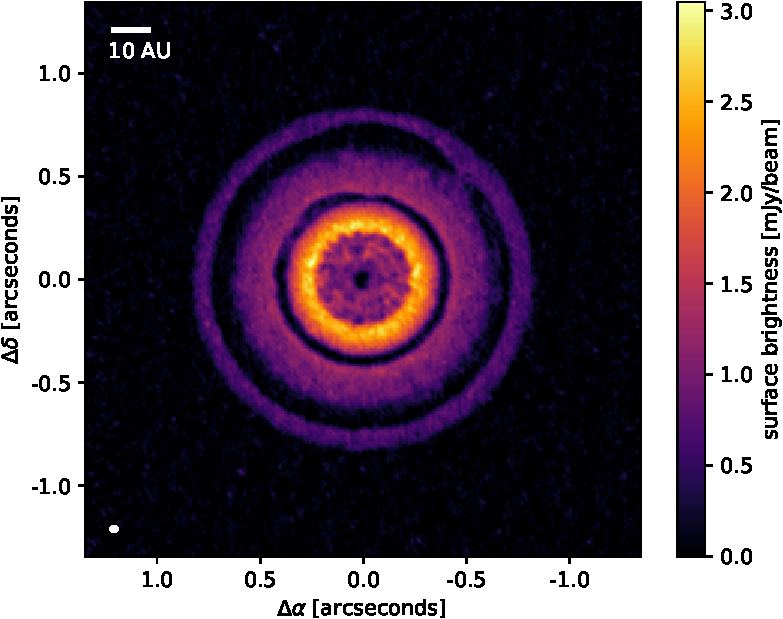
\includegraphics[width=0.32\columnwidth]{figs/total-to-SPH-dust_20.pdf}
      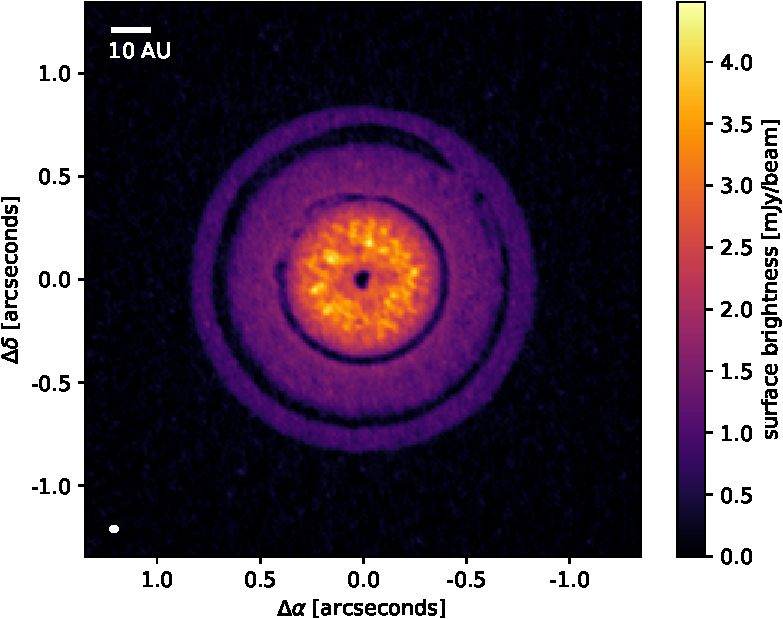
\includegraphics[width=0.32\columnwidth]{figs/total-to-SPH-dust_100.pdf}
      \caption{Total dust to SPH dust ratio: 10, 20, 100 from
         \texttt{2017-06-27a}, cycle 3.8, 45 minute observing time.}
      \label{fig:sph-dust-mass}
   \end{center}
\end{figure}

\begin{figure}
   \begin{center}
      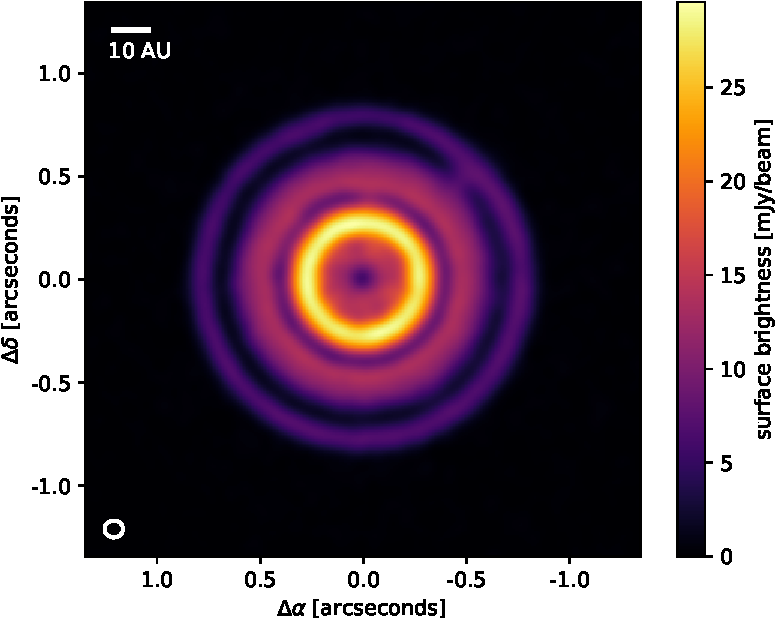
\includegraphics[width=0.32\columnwidth]{figs/cycle3.6.pdf}
      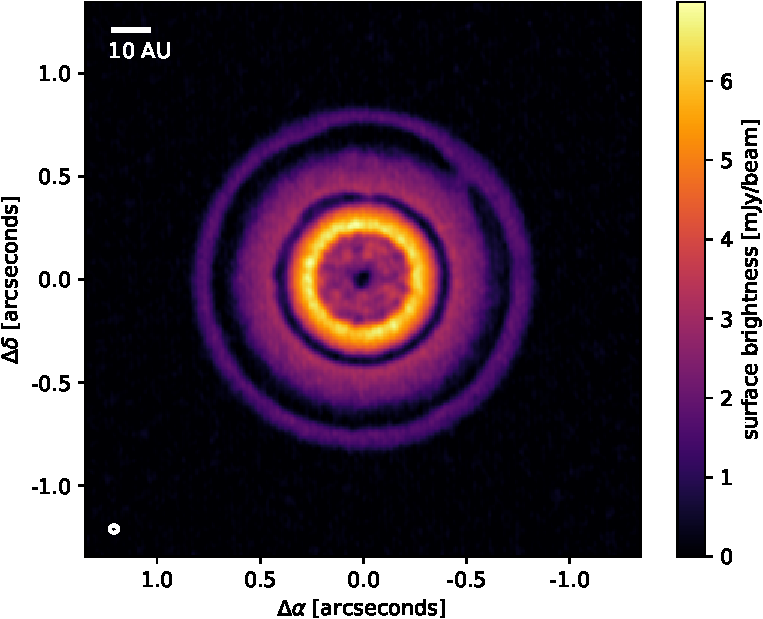
\includegraphics[width=0.32\columnwidth]{figs/cycle3.7.pdf}
      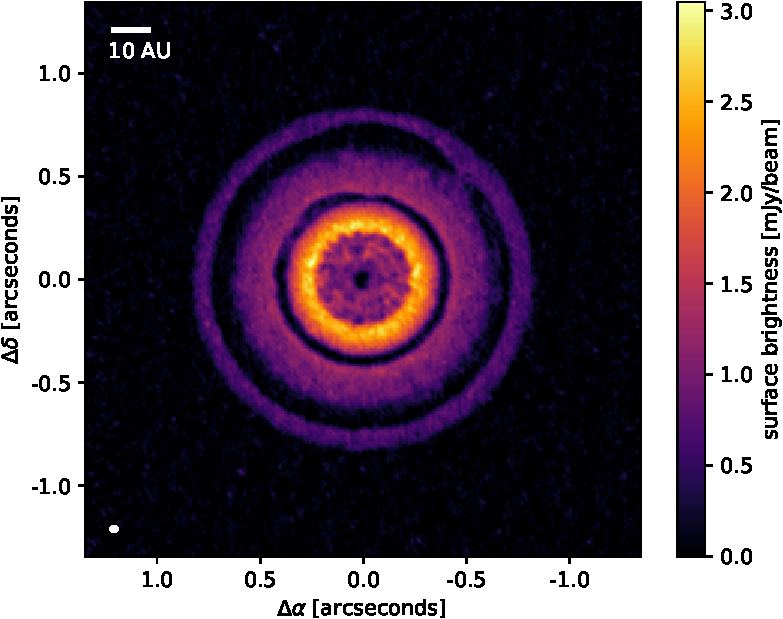
\includegraphics[width=0.32\columnwidth]{figs/cycle3.8.pdf}
      \caption{Varying beam size: ALMA cycle 3.6, 3.7, 3.8 from
         \texttt{2017-06-27a}, 45 minute observing time.}
      \label{fig:beam-size}
   \end{center}
\end{figure}


\section*{\texttt{dtdrag} and Stokes number on particles (\texttt{2017-08-01})}

See Figs.~\ref{fig:dtdrag}, ~\ref{fig:sph-dust-gas-particle-ratio},
~\ref{fig:accretion-problems}.


\subsection*{Speed up}

The speed up is by increasing number of gas particles relative to the number of
dust particles. This seems to keep the dust particles from clumping leading to
high dust density and thus low Stokes number reducing the drag time step
constraining the time stepping. Here are some timings (for an inner disc radius
at 10~au we have that):
\begin{itemize}
   \item 1M + 100K takes 236~hours for 70 orbits (20000~years). Extrapolating
      gives 700~hours or 29~days for 200 orbits. From \texttt{2017-07-07a}.\\
   \item 2M + 50K takes 142~hours for 200 orbits (59000~years). This gives
      142~hours or 6~days for 200 orbits. From \texttt{2017-08-08a}.\\
   \item 10M + 250K takes 150~hours for 40 orbits (12000~years). Extrapolating
      gives 750~hours or 31~days for 200 orbits. From \texttt{2017-08-09a}.
\end{itemize}

\noindent\textit{The following table is the wall time taken to reach 200 orbits
at 41~au (59,000 yrs) for an inner disc radius at 10~au.}
\begin{center}
   \begin{tabular}{ l c c }
      \hline
      1M + 100K  & 700 hr & 29 days \\
      2M + 50K   & 150 hr & 6 days \\
      10M + 250K & 750 hr & 31 days
      \hline
   \end{tabular}
\end{center}

I believe that this speed up is due to a lack of dust getting trapped under the
gas resolution and going to high density and thus making the dust drag time go
small.


\begin{figure}
   \begin{center}
      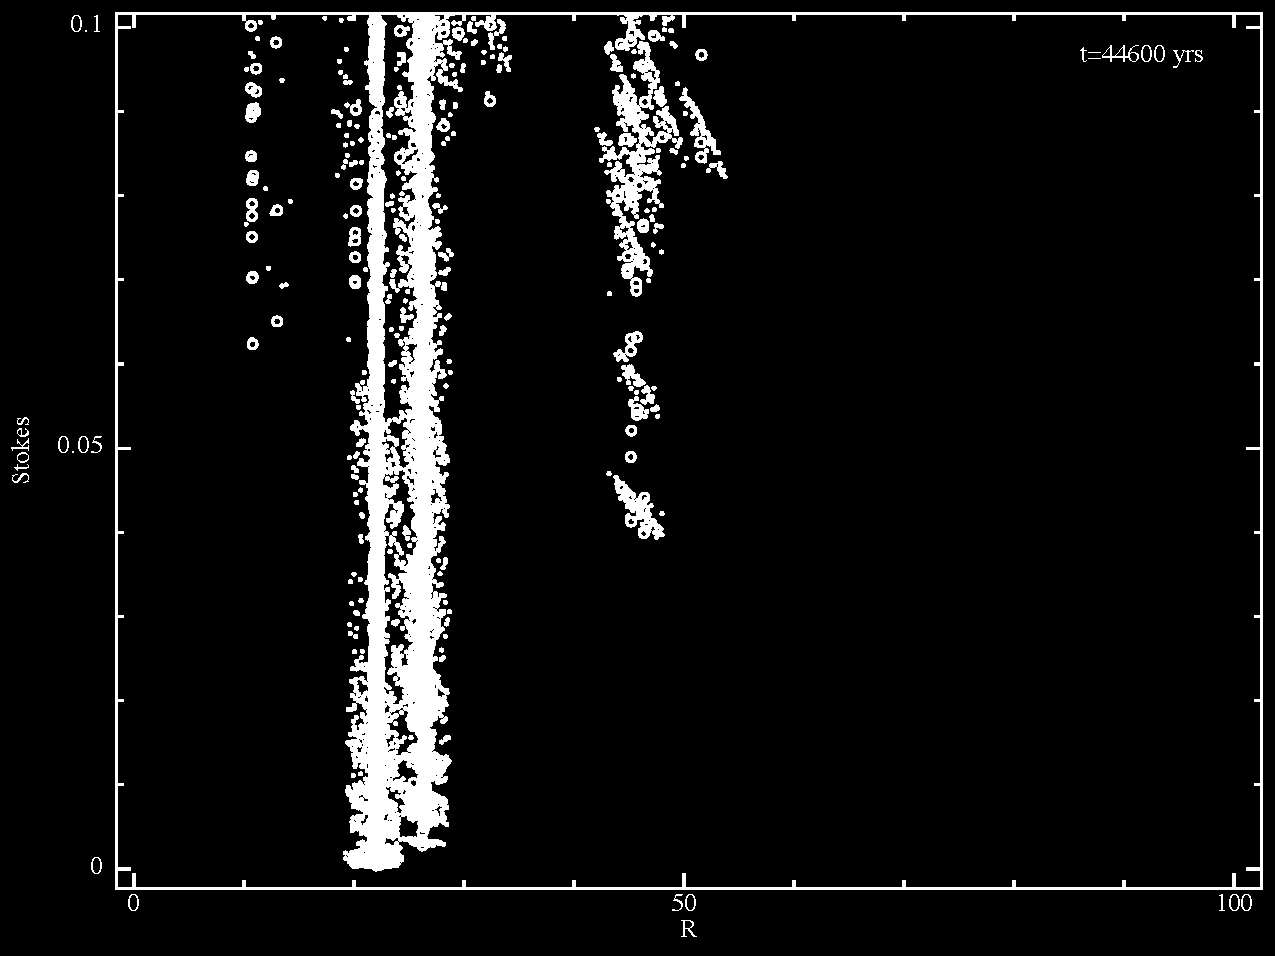
\includegraphics[width=0.48\columnwidth]{figs/dtdrag_bad.pdf}
      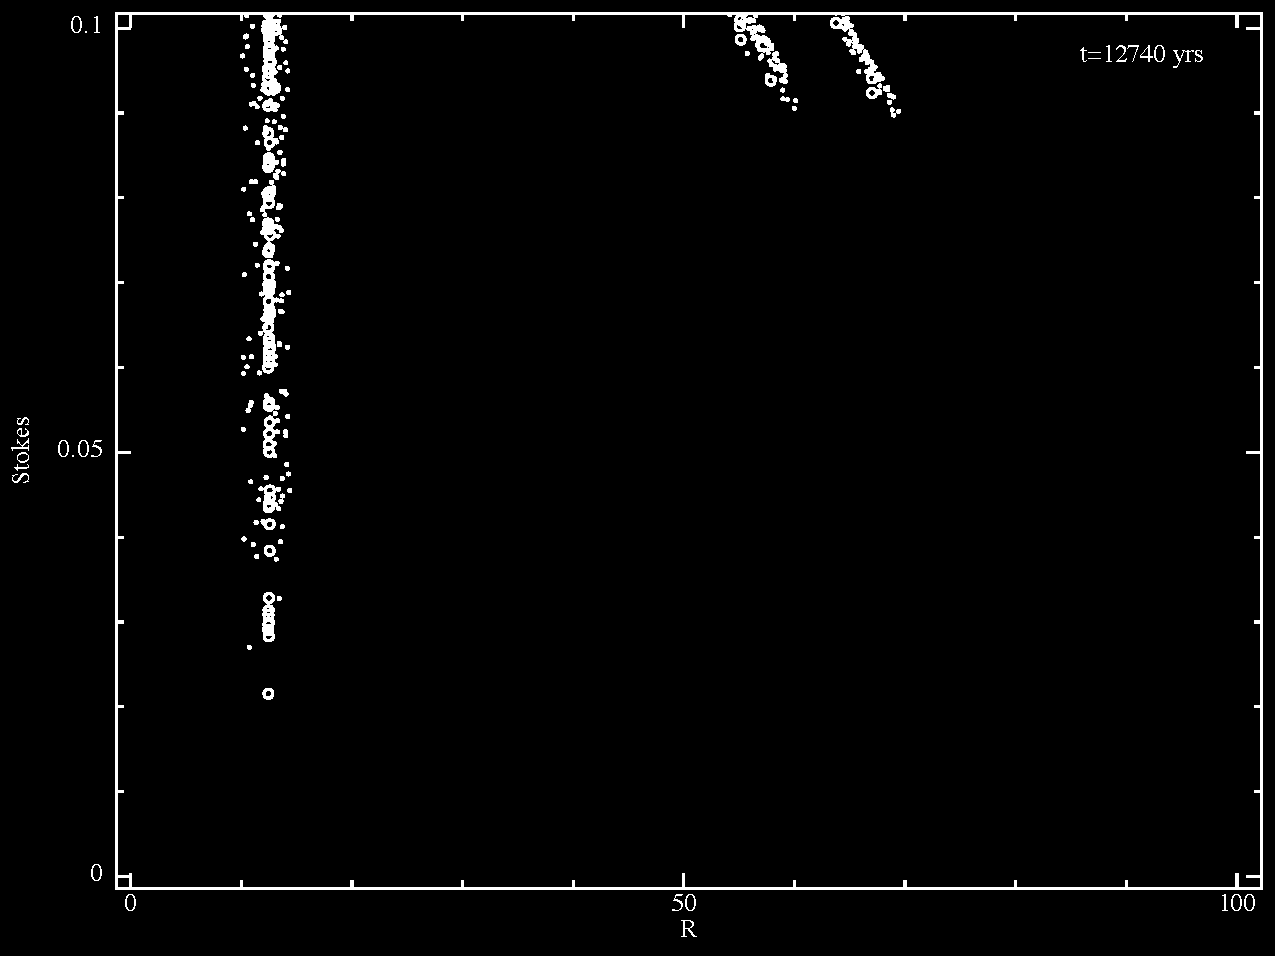
\includegraphics[width=0.48\columnwidth]{figs/dtdrag_good.pdf}\\
      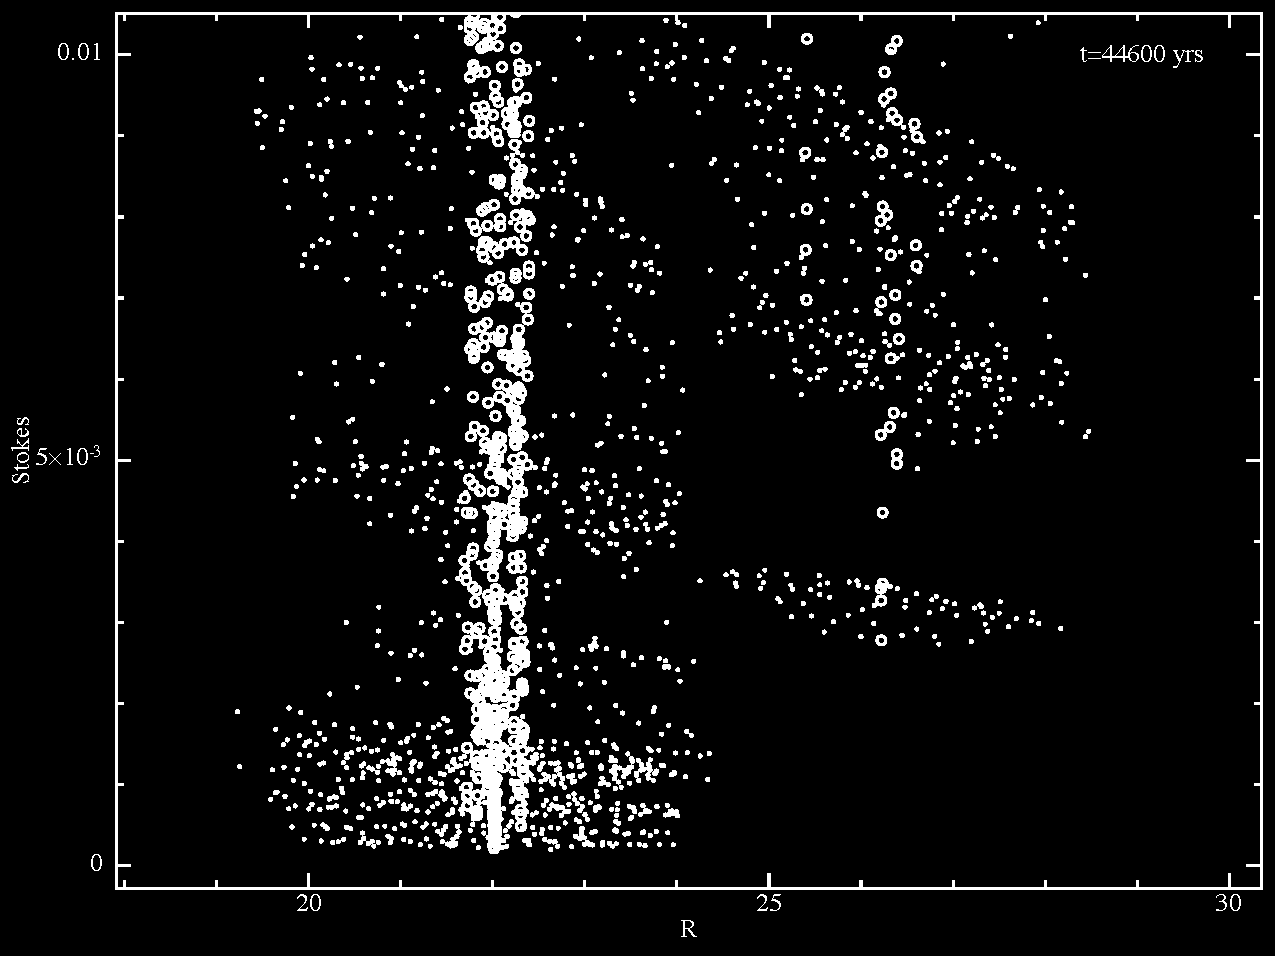
\includegraphics[width=0.48\columnwidth]{figs/dtdrag_bad_zoomed.pdf}
      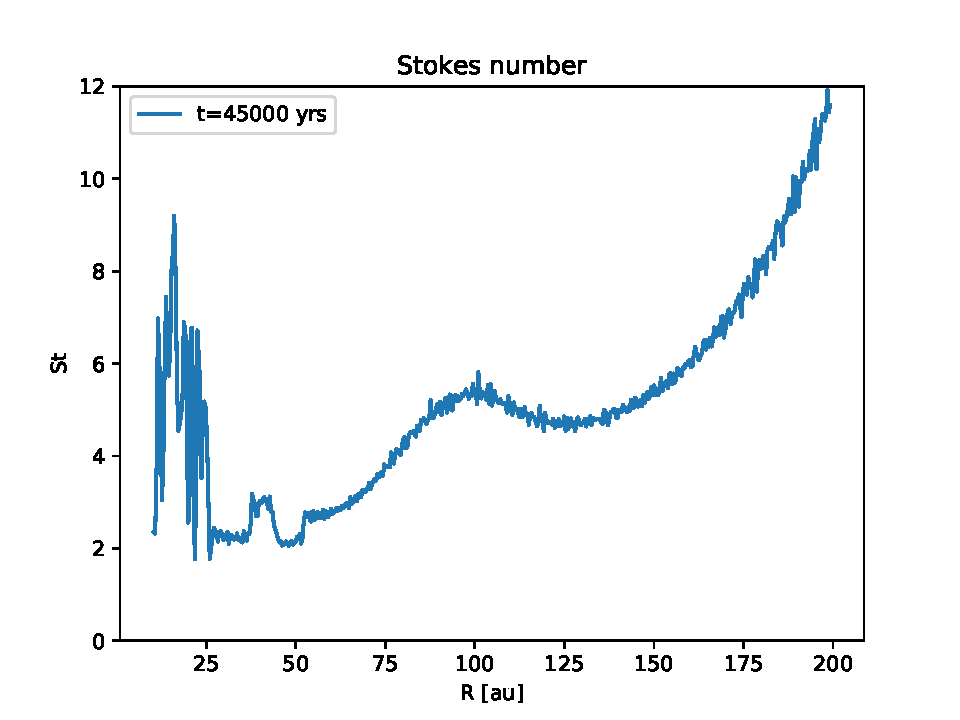
\includegraphics[width=0.48\columnwidth]{figs/dtdrag_Stokes_bad.pdf}\\
      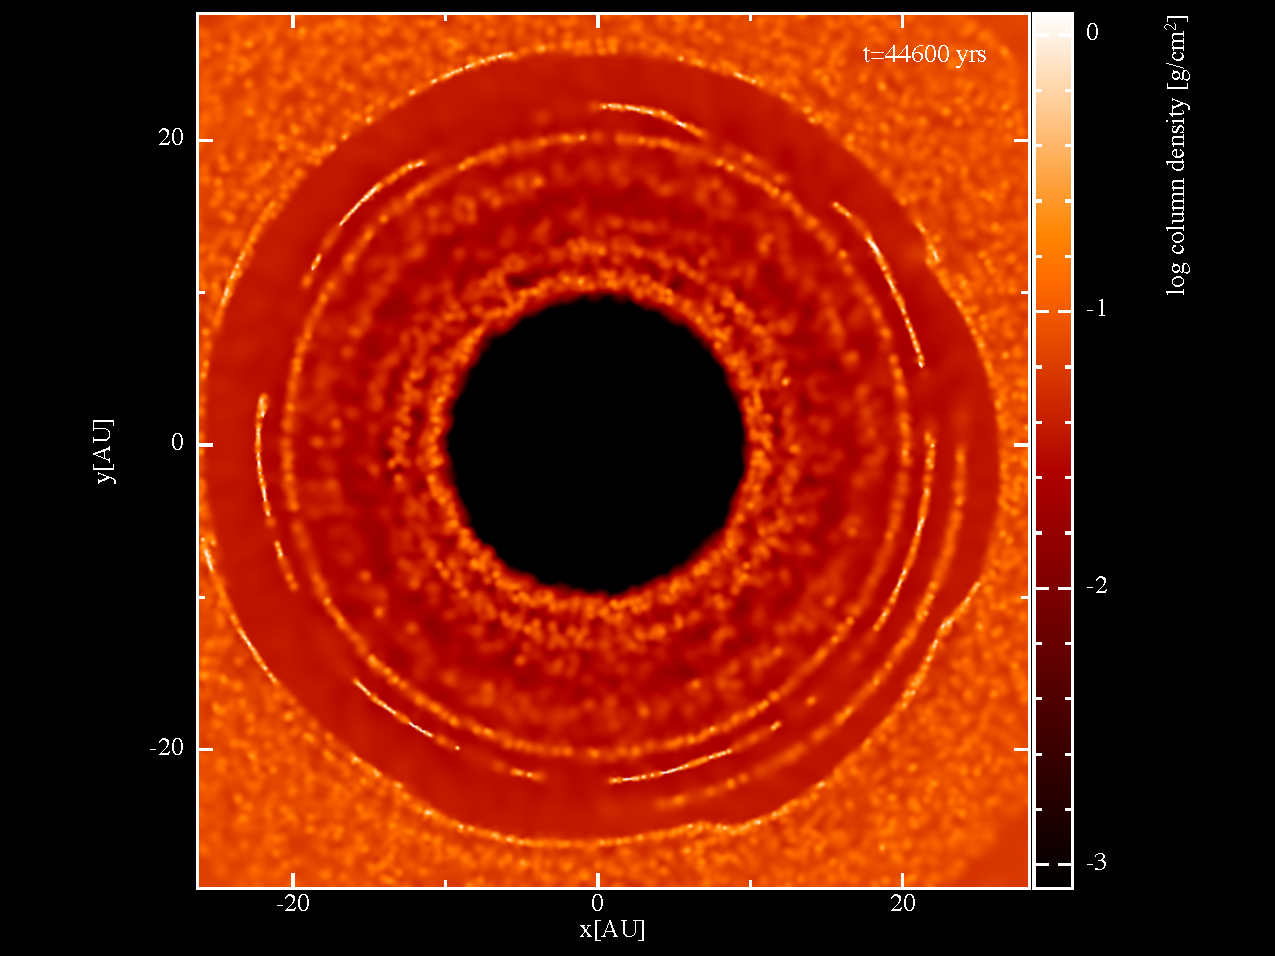
\includegraphics[width=0.48\columnwidth]{figs/dtdrag_bad_density.pdf}
      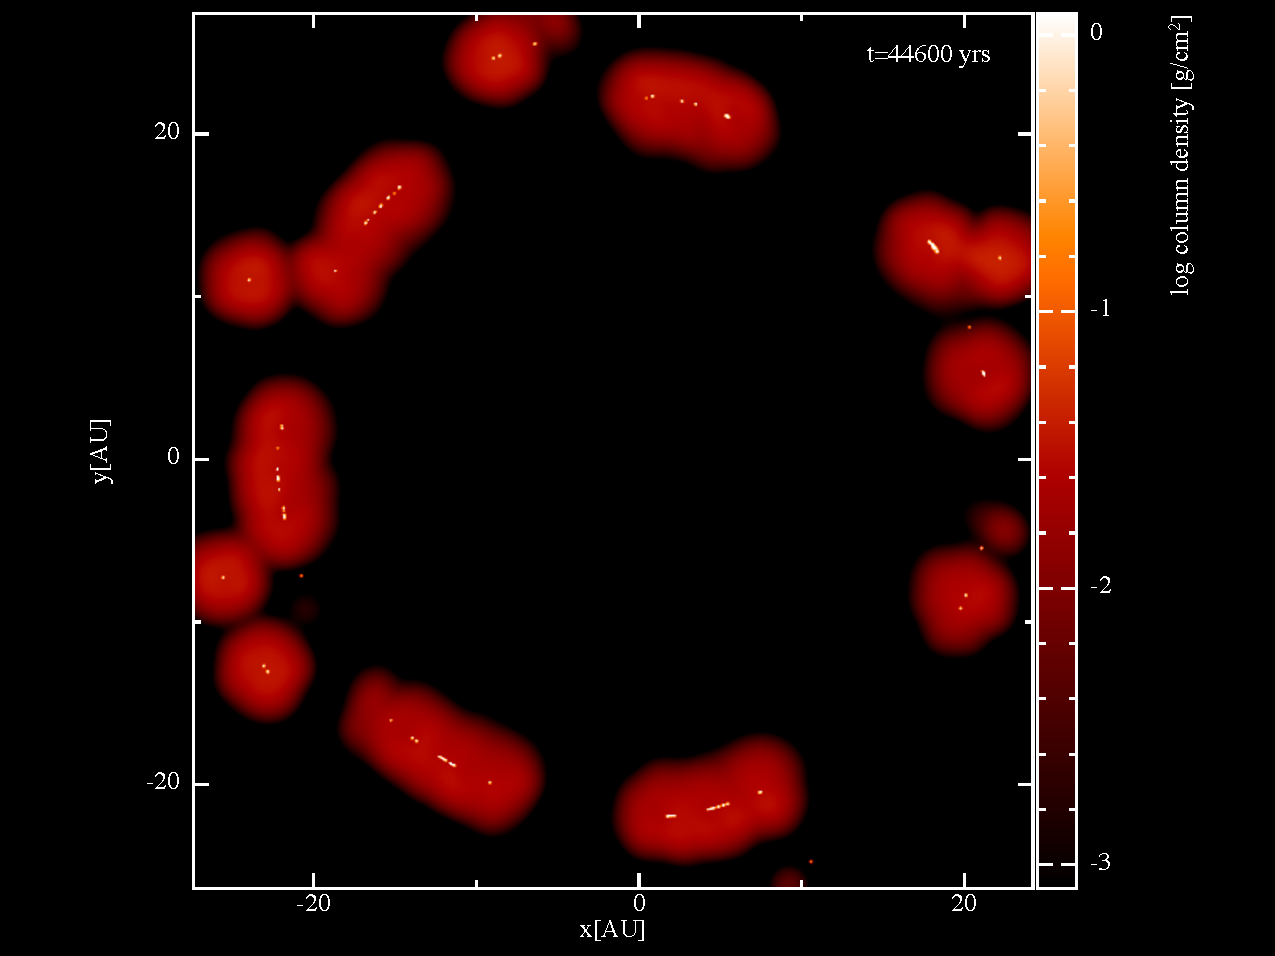
\includegraphics[width=0.48\columnwidth]{figs/dtdrag_bad_density_low_Stokes_particles.pdf}
      \caption{\textit{Top left}: at late times (dump 175) \texttt{dtdrag}
         constrains step size due to many particles with Stokes number less than
         $\sim 0.1$ (smallest $\sim 10^{-4}$); \textit{top right}: at earlier
         times (dump 50) the constraint is not so bad (not many particles with
         small Stokes number, and smallest Stokes $\sim 10^{-2}$).
         \textit{Middle left}: zoomed in from above; \textit{middle right}:
         azimuthally averaged Stokes number for later time (same as top left)
         where we see that the Stokes number should be above unity everywhere.
         \textit{Bottom left}: dust and gas density---note the thin high density
         regions within the dust gap; \textit{bottom right}: same as left but
         only particles with small Stokes number are plotted---they coincide
         with the high density regions on the left. From
      \texttt{2017-07-07a}.}
      \label{fig:dtdrag}
   \end{center}
\end{figure}

\begin{figure}
   \begin{center}
      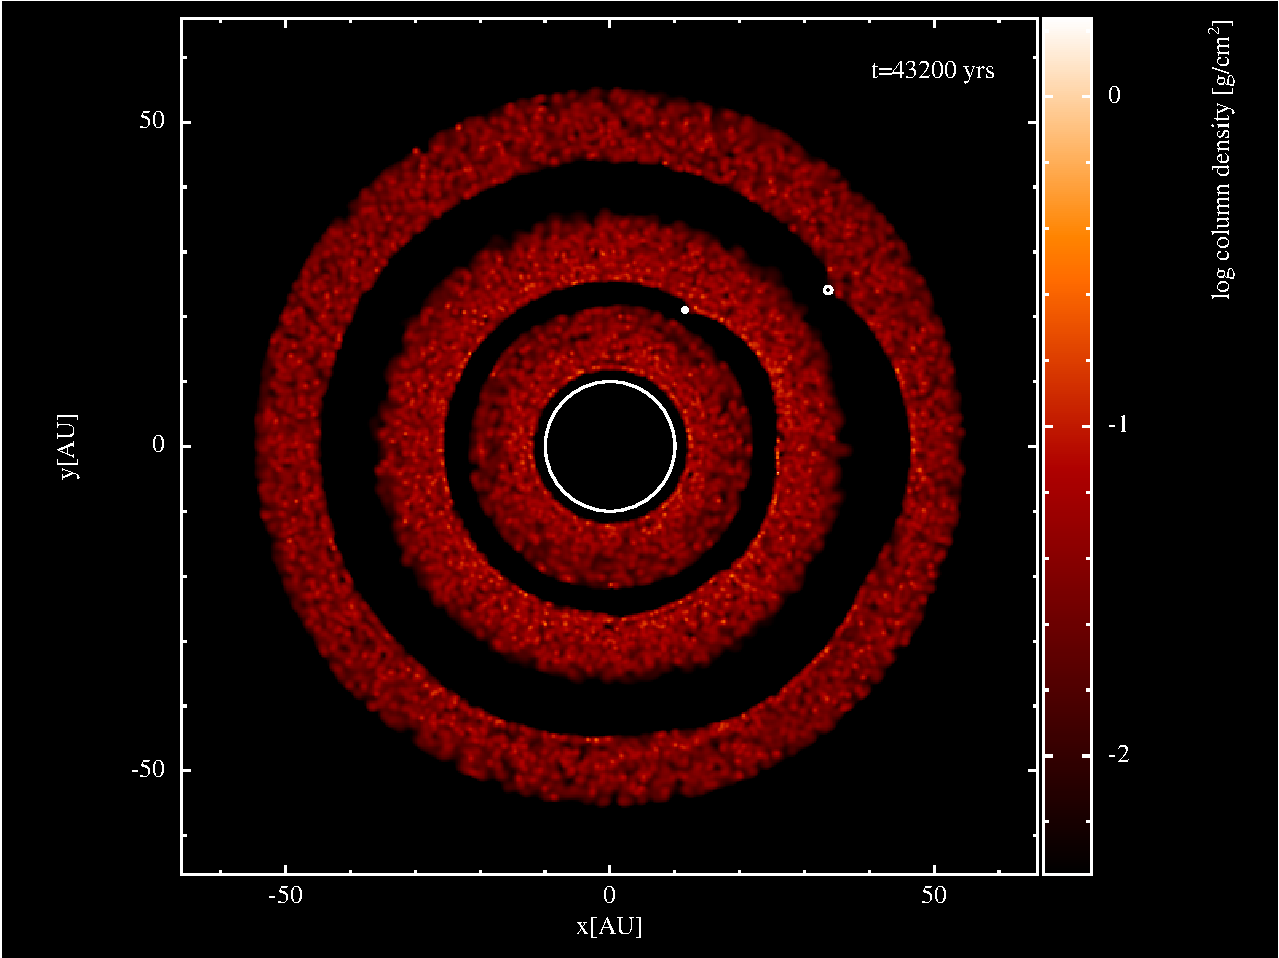
\includegraphics[width=0.48\columnwidth]{figs/sph-dust-gas-particle-ratio-dust.pdf}
      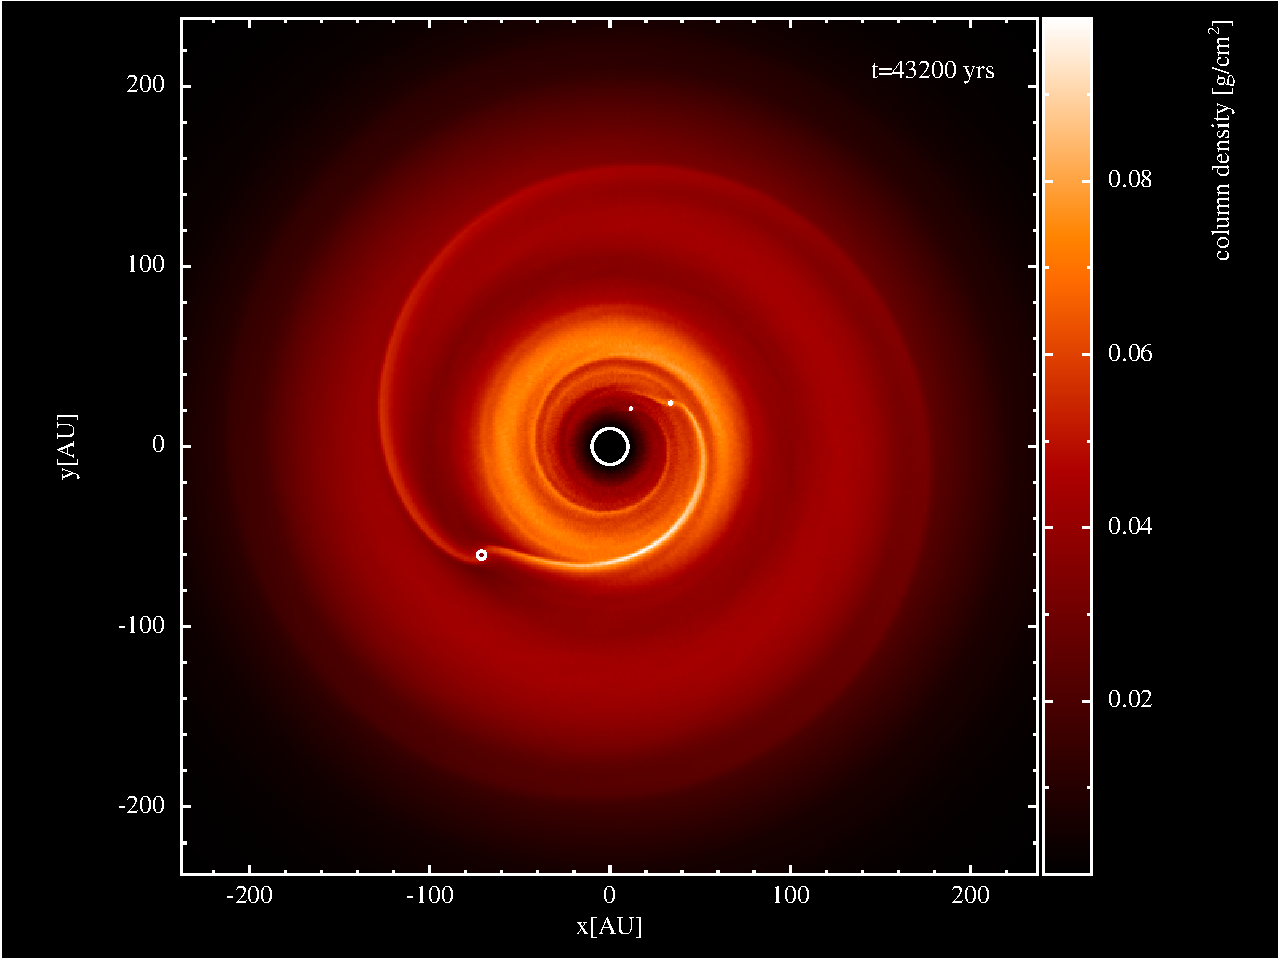
\includegraphics[width=0.48\columnwidth]{figs/sph-dust-gas-particle-ratio-gas.pdf}
      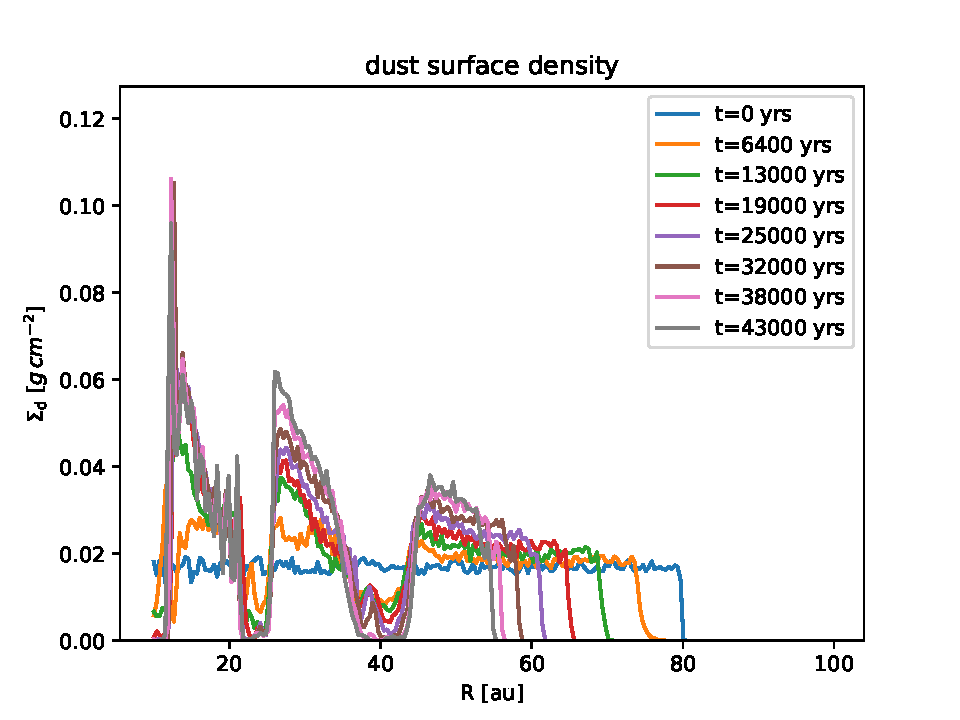
\includegraphics[width=0.48\columnwidth]{figs/sph-dust-gas-particle-ratio-dust-sigma.pdf}
      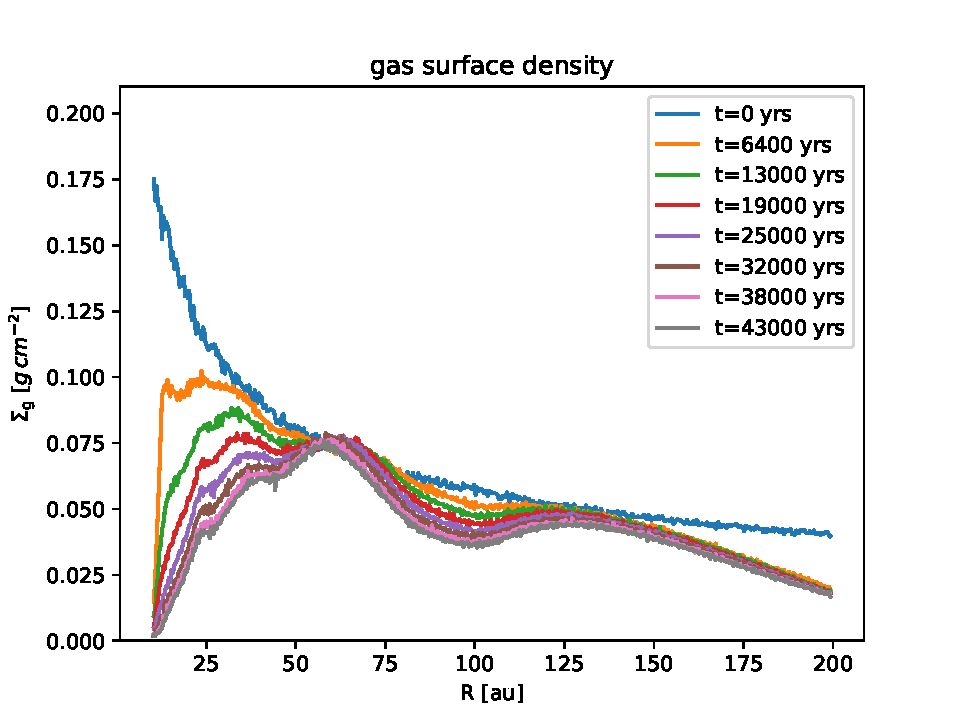
\includegraphics[width=0.48\columnwidth]{figs/sph-dust-gas-particle-ratio-gas-sigma.pdf}
      \caption{Increased ratio of gas to dust SPH particle number: 2M gas + 50K
      dust. From \texttt{2017-08-03a/00678}. 16~M${}_{\oplus}$ planets.}
      \label{fig:sph-dust-gas-particle-ratio}
   \end{center}
\end{figure}

\begin{figure}
   \begin{center}
      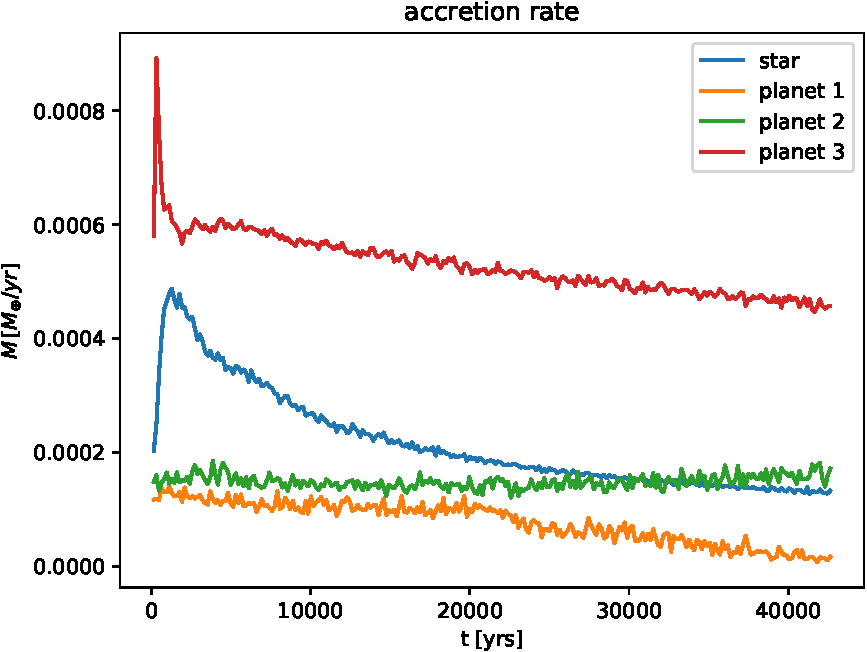
\includegraphics[height=0.35\columnwidth]{figs/mdot_2017-08-03a.pdf}
      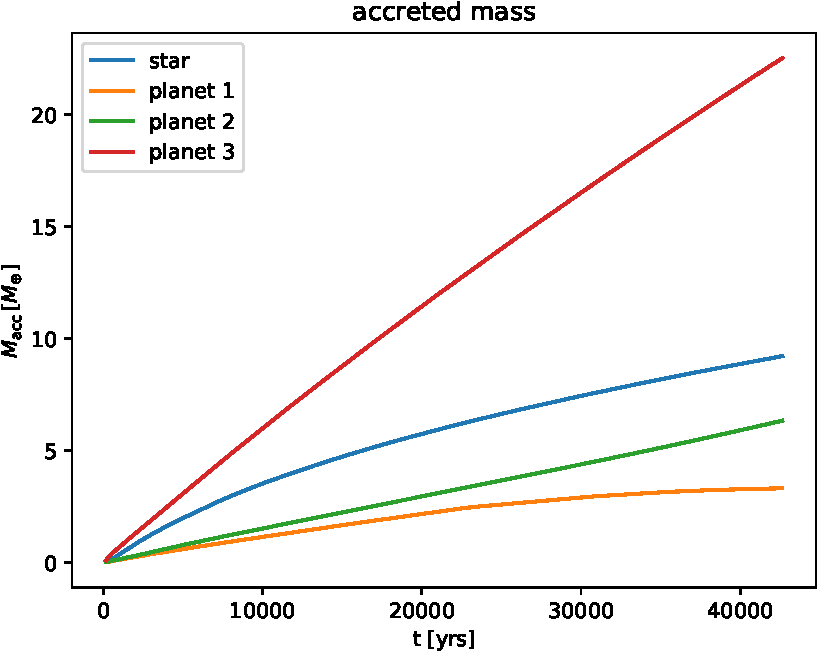
\includegraphics[height=0.35\columnwidth]{figs/macc_2017-08-03a.pdf}
      \caption{Accretion problems (update: what problems?). From
      \texttt{2017-08-03a}.}
      \label{fig:accretion-problems}
   \end{center}
\end{figure}


\section*{Dust gap width sensitivity on resolution (\texttt{2017-08-20})}

See Fig.~\ref{fig:gap-width-resolution}.

\begin{figure}
   \begin{center}
      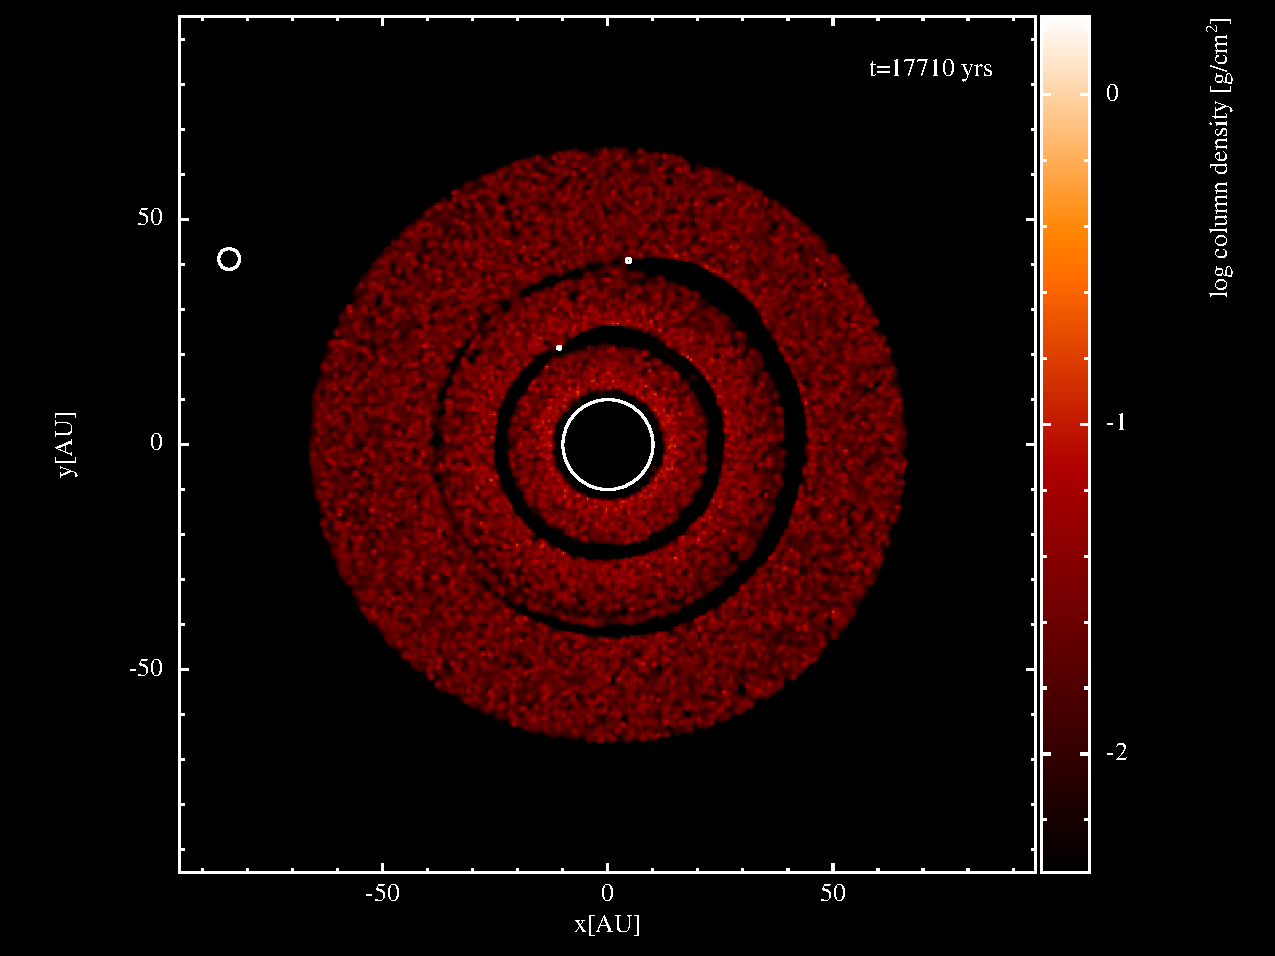
\includegraphics[width=0.48\columnwidth]{figs/dust_gap_low_resolution.pdf}
      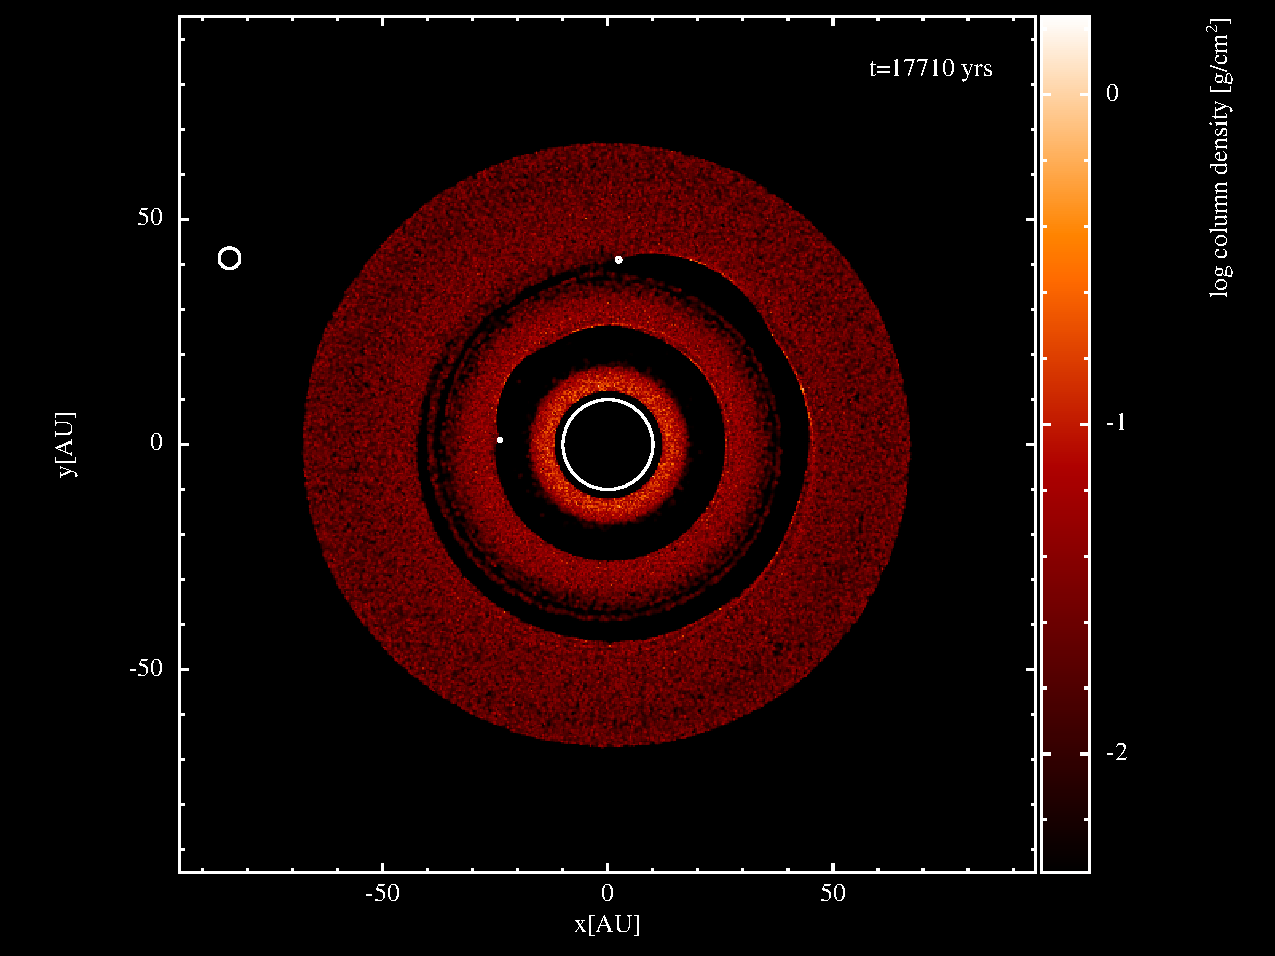
\includegraphics[width=0.48\columnwidth]{figs/dust_gap_high_resolution.pdf}
      \caption{Dust gap width sensitivity on resolution. Gap width seems to be
         sensitive to resolution. Both figures are same physical parameters.
         Except viscosity. They have the same artificial viscosity. So given
         that one has 5 times as many particles as the other the
         $\alpha$-viscosity is different by a factor $\sqrt[3]{5}$.
         Note: the low resolution calculation has 2M gas + 50K dust; high
         resolution has 10M gas + 250K dust. From \texttt{2017-08-08a/00139}
         and \texttt{2017-08-09a/00139}.}
      \label{fig:gap-width-resolution}
   \end{center}
\end{figure}



\section*{Planet mass comparison (\texttt{2018-03-05})}

See Fig.~\ref{fig:planet-mass-comparison}.

\begin{figure*}
   \begin{center}
      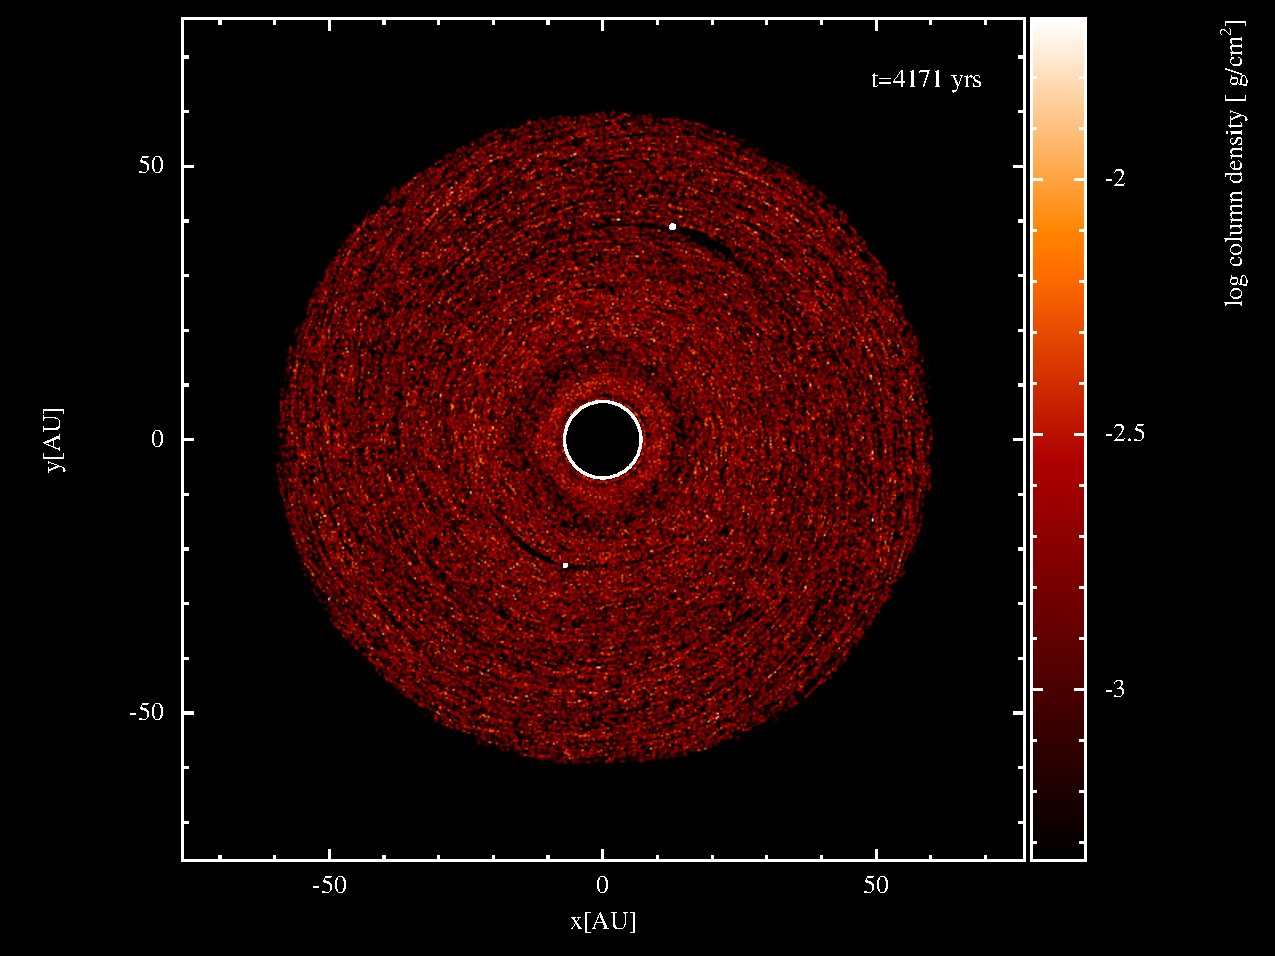
\includegraphics[width=0.32\textwidth]{figs/4-100mu-dust.pdf}
      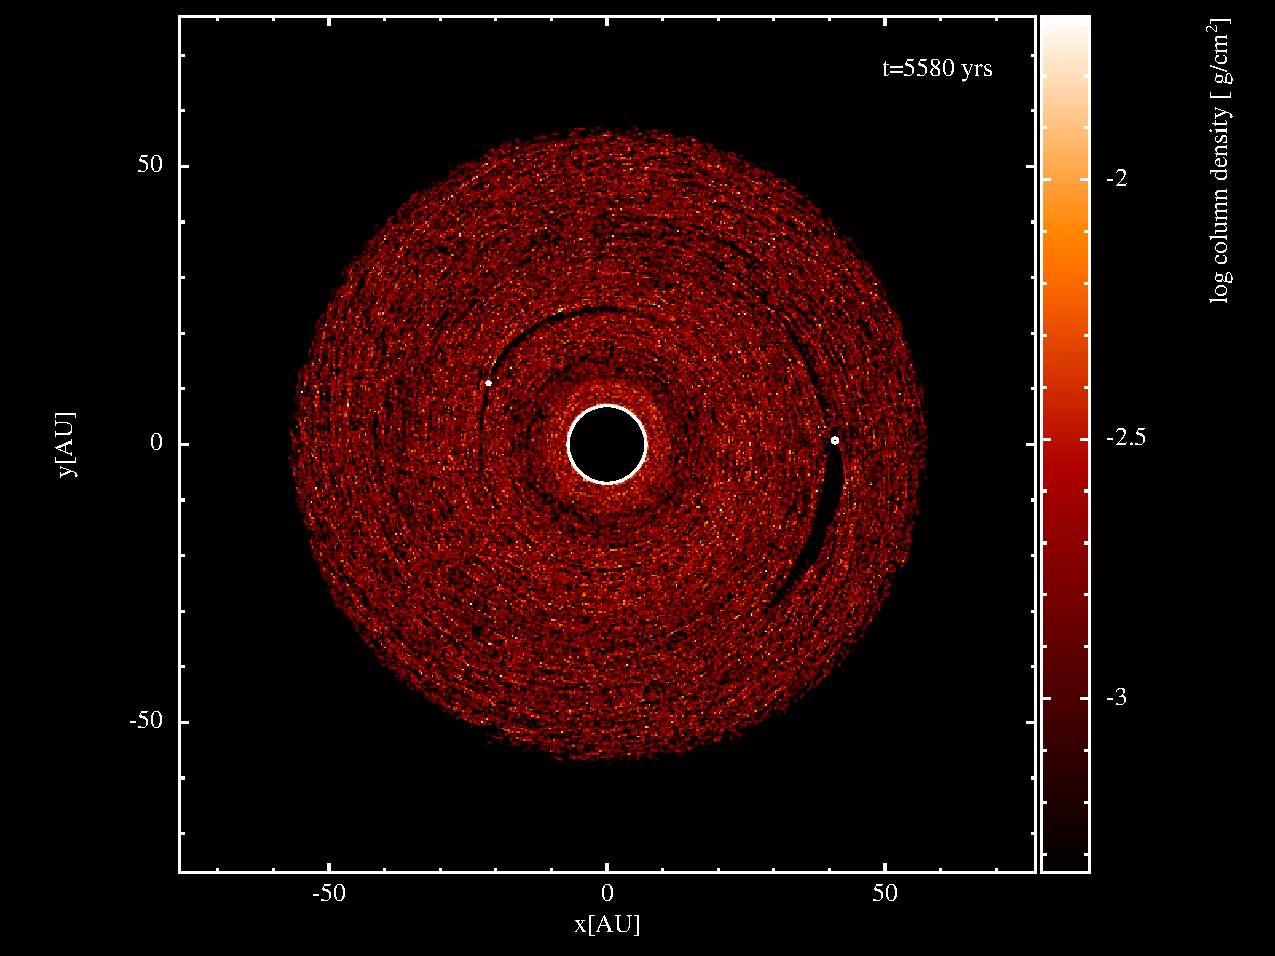
\includegraphics[width=0.32\textwidth]{figs/8-100mu-dust.pdf}
      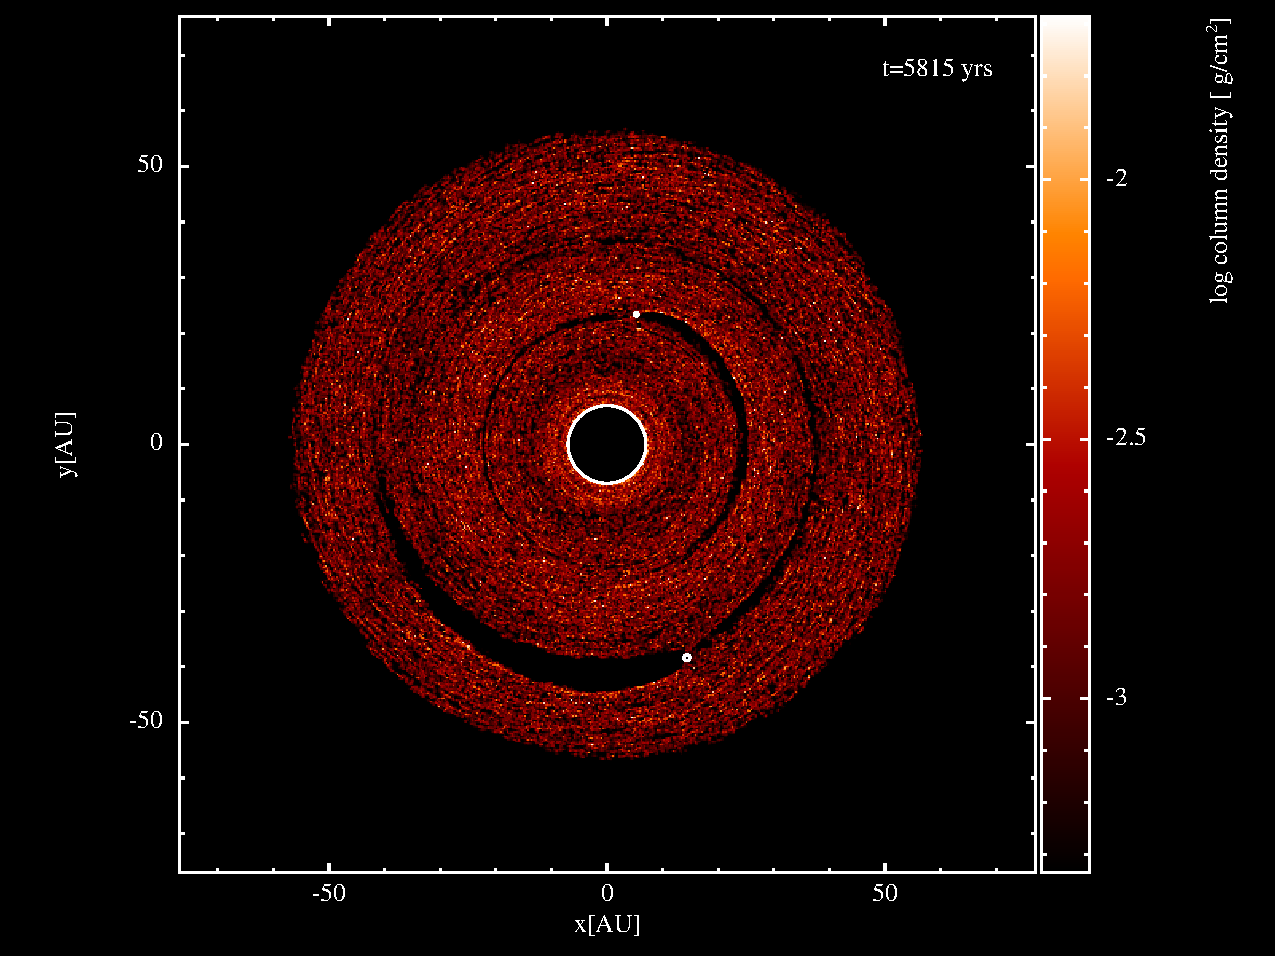
\includegraphics[width=0.32\textwidth]{figs/16-100mu-dust.pdf}
      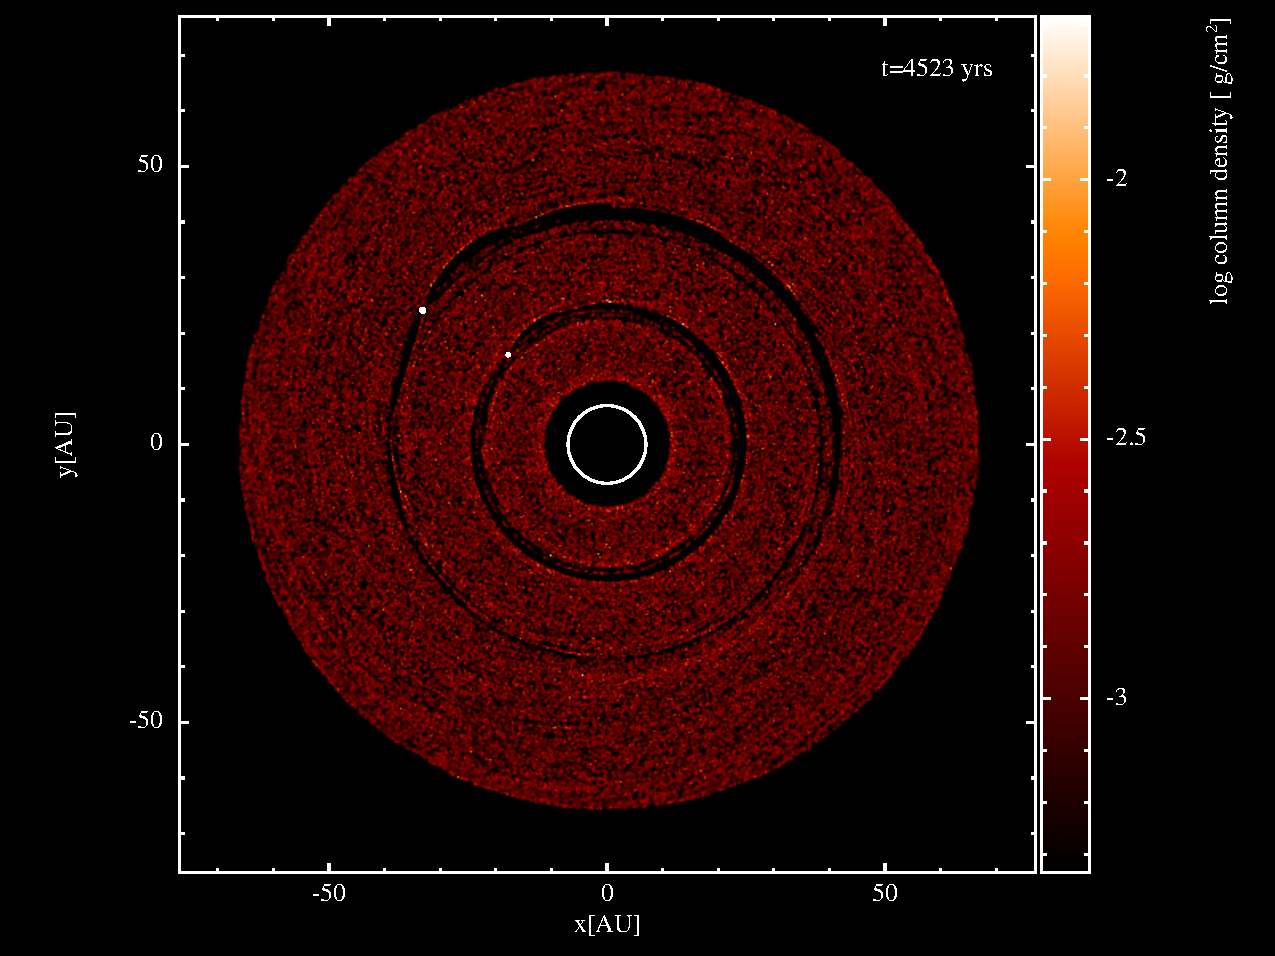
\includegraphics[width=0.32\textwidth]{figs/4-1mm-dust.pdf}
      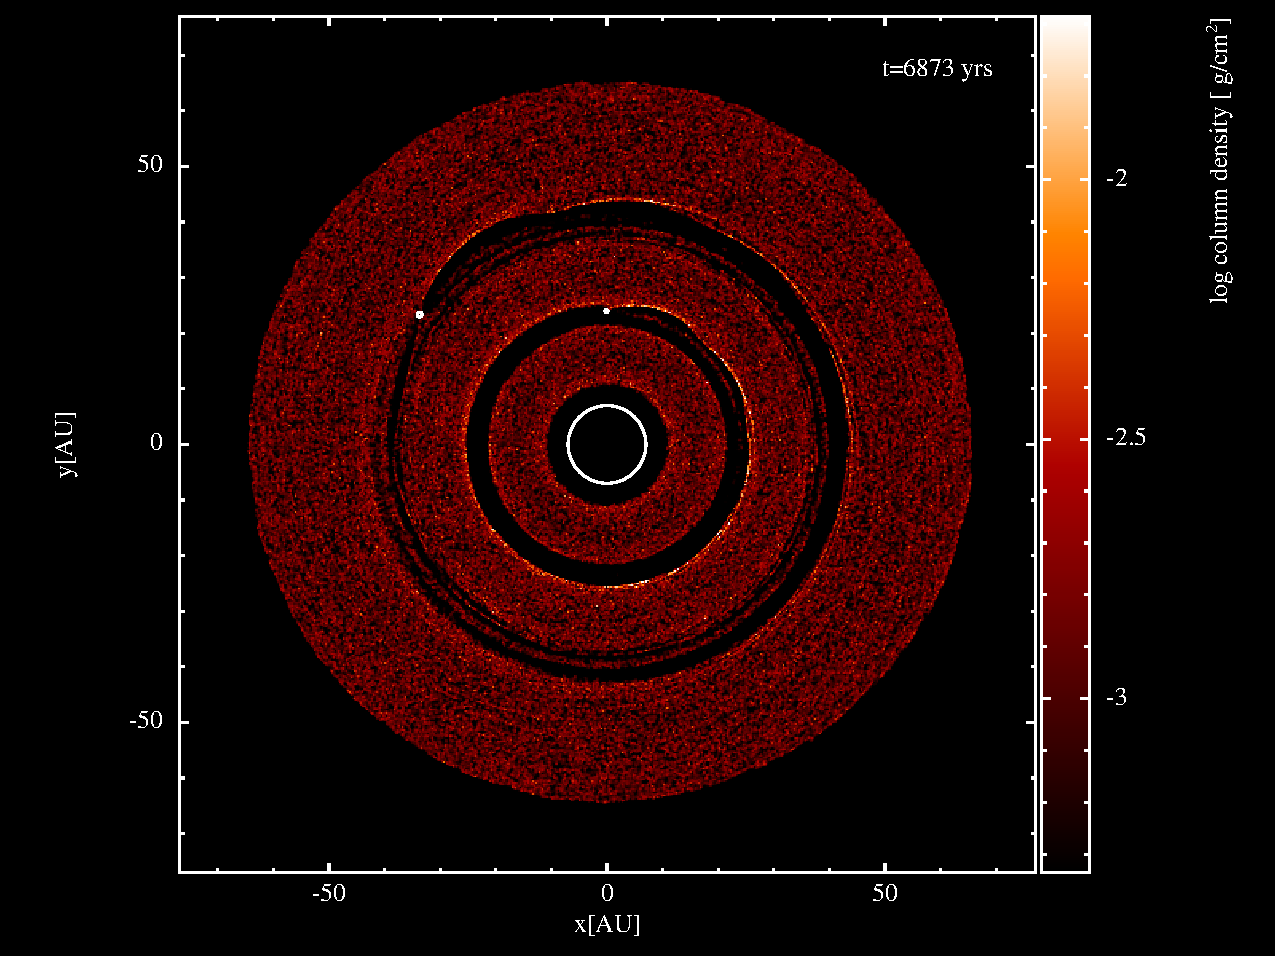
\includegraphics[width=0.32\textwidth]{figs/8-1mm-dust.pdf}
      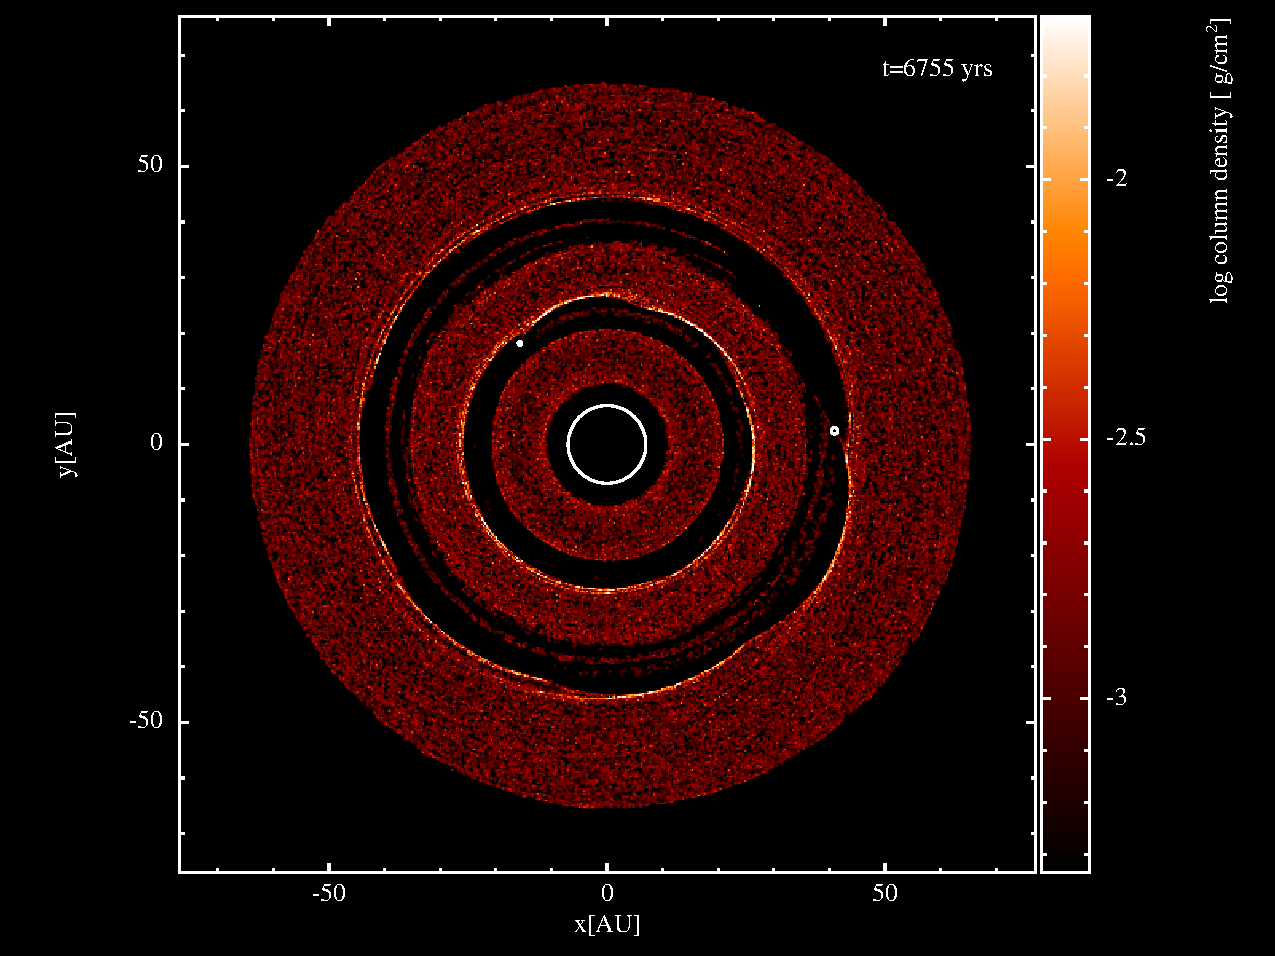
\includegraphics[width=0.32\textwidth]{figs/16-1mm-dust.pdf}
      \caption{Left to right: 4, 8, 16~$\earth{}$. Top: 100~$\mu$m. Bottom
      1~mm. $\alpha_{AV}=0.2$, $\alpha_{SS}\approx0.005$. 500K + 300K. ALMA
      region only ($R_{\mathrm{out,g}} = 90$~au, $R_{\mathrm{out,d}} = 70$~au).}
      \label{fig:planet-mass-comparison}
   \end{center}
\end{figure*}





\section*{Planet mass comparison (\texttt{2018-04-23})}

See Fig.~\ref{fig:planet-mass-comparison2} for a comparison after ALMA
processing.

\begin{figure*}
   \begin{center}
      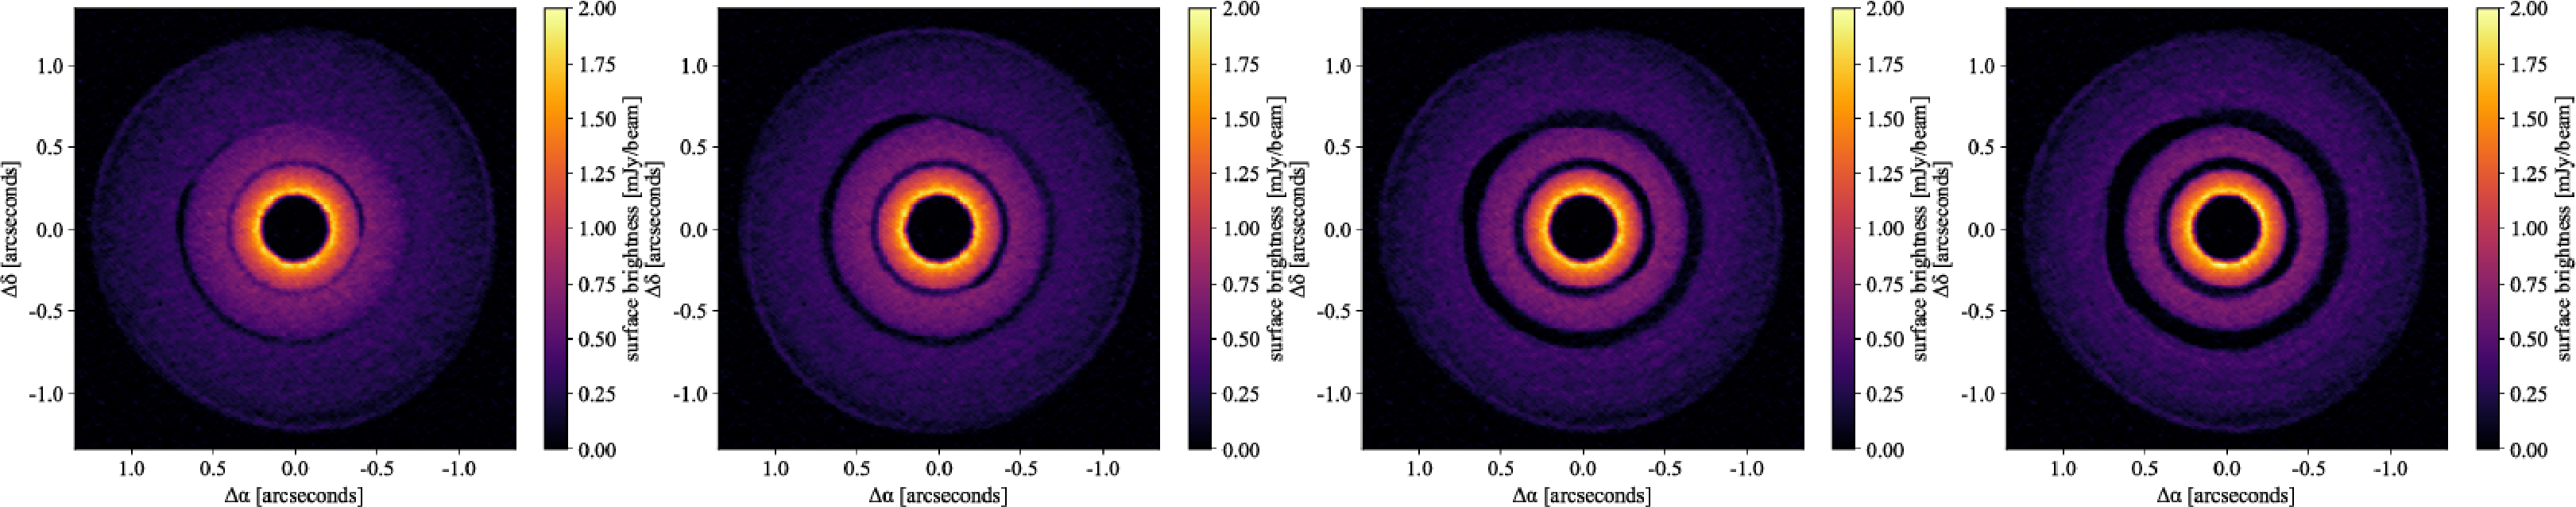
\includegraphics[width=0.98\textwidth]{figs/planet-mass-comparison-alma-100.pdf}
      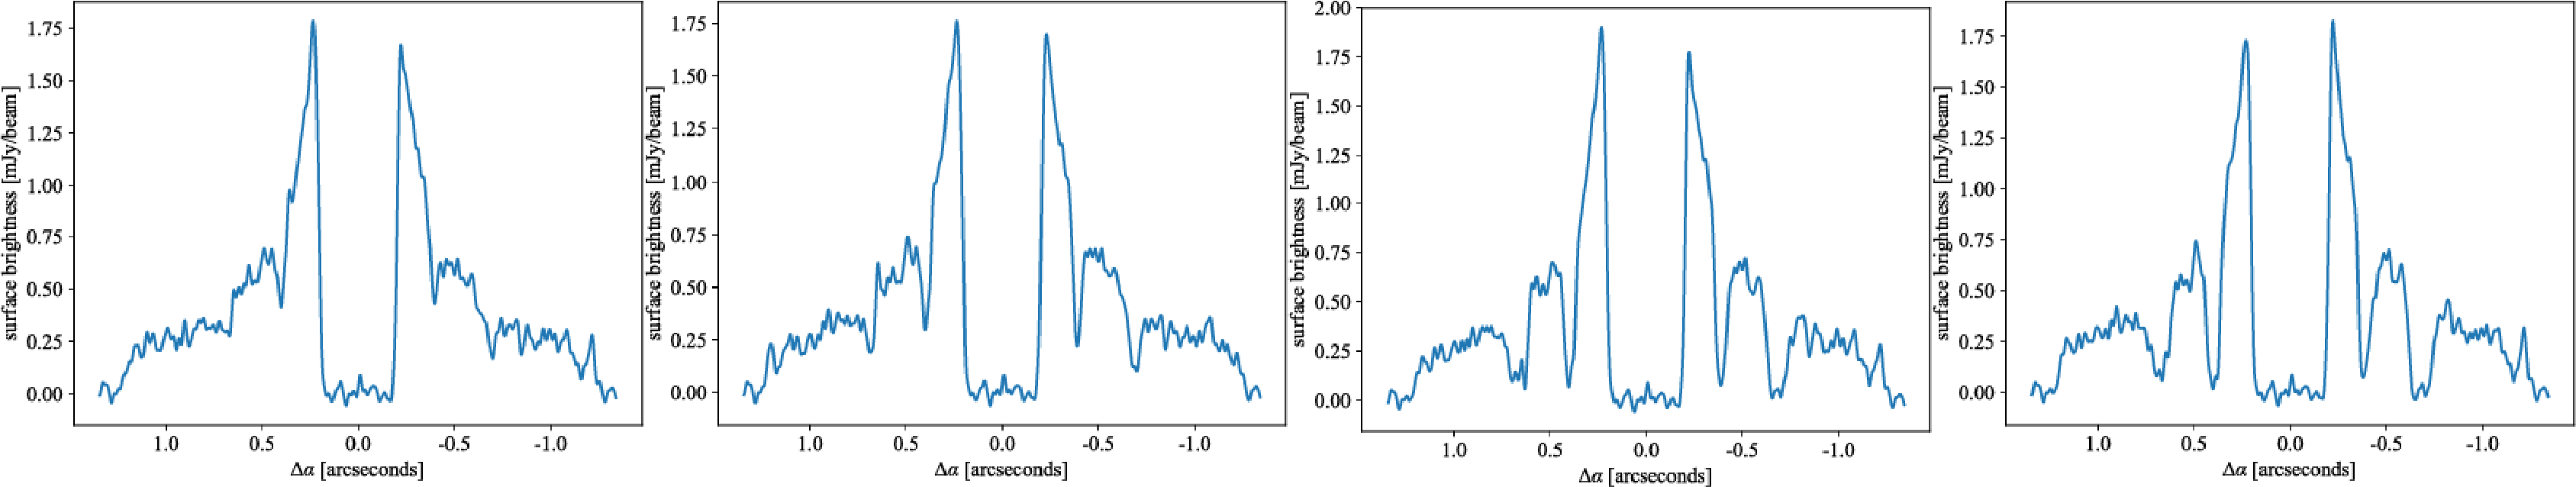
\includegraphics[width=0.98\textwidth]{figs/planet-mass-comparison-alma-100-radial-cut.pdf}
      \caption{Planet masses: 4, 8, 16, 24~$\earth{}$. 100~$\mu$m grains. 10M +
      250K. See runs: \texttt{2018-03-\{02b,12a,02a,13a\}/00125}.}
      \label{fig:planet-mass-comparison2}
   \end{center}
\end{figure*}




\end{document}
